\documentclass[12pt]{article}
\usepackage{config}
\usepackage{subfiles}

\begin{document}

\begin{flushright}
    Конспект Шорохова Сергея

    Если нашли опечатку/ошибку - пишите @le9endwp
\end{flushright}

\tableofcontents
\newpage

\section{Линейная алгебра и геометрия}

Типичная система линейных уравнений: $\left\{\begin{array}{l}
    ax + by = e \\
    cx + dy = f
\end{array}\right.;\ a, b, c, d, e, f \in R$ -- кольцо или $\in K$ -- поле

Неизвестные здесь: ${x \choose y} \in K \times K$

Множество линейных уравнений: $\{ px + qy = r \}$

Операции:

\begin{itemize}
    \item Их можно складывать
    \item Умножать на константу (элемент $K$)
\end{itemize}

\vspace{5mm}

\begin{defin}{Векторное пространство}
    $K$ -- поле. Векторное пространство над $K$ это $(V, +, \cdot)$, где V -- множество, $+: V \times V \rightarrow V$, $\cdot: K \times V \rightarrow V$
\end{defin}

\vspace{5mm}

\textbf{Аксиомы:}

\begin{enumerate}
    \item[1-4.] $(V, +)$ -- абелева группа
    \item[5.] $(ab)v = a(bv)\ \forall a, b \in K, v \in V$
    \item[6.] $(a + b)v = av + bv\ \forall a, b \in K, v \in V$
    \item[7.] $a(v + u) = av + au\ \forall a \in K, v, u \in V$
    \item[8.] $1v = v\ \forall v \in V$
\end{enumerate}

\vspace{5mm}

\begin{lem}{}
    $0 \cdot v = \overrightarrow{0}\ \forall v \in V$

    $(-1) \cdot v = -v\ \forall v \in V$
\end{lem}

\textit{Доказательство:}

$(0 + 0)v = 0v + 0v \Rightarrow 0v = 0v + 0v$

$(-0)v + 0v = (-0)v + 0v + 0v \Rightarrow \overrightarrow{0} = 0v$

Тогда $\overrightarrow{0} = 0v = (1 + (-1))v = 1v + (-1)v = v + (-1)v$, т.е. $v + (-1)v = \overrightarrow{0} \Rightarrow (-1)v = -v$

\begin{Remark}{}
    $u + v = v + u\ \forall u, v \in V$ следует из остальных 7 аксиом пространства (упражнение)
\end{Remark}

\begin{Example}{}
    Тут рисуночки, говорящие что два вектора задают пространство, в котором выполнены аксиомы 1-8

    Заметим, что есть биекция $vec \leftrightarrow R^2$, т.е. $v \rightarrow {a \choose b}$
\end{Example}

\begin{Example}{Самый главный пример}
    $K^n = \{\left( \begin{gathered}
        a_1 \\
        a_2 \\
        \vdots \\
        a_n
    \end{gathered} \right) | a_i \in K\}$

    А еще тут выполнены все аксиомы (доказано методом очев): можем складывать, домножать итд

    Это называем пространство столбцов

    \vspace{3mm}

    $^nK = \{ (a_1, a_2 \ldots a_n) | a_i \in K\}$

    А это то же самое, но называем пространством строк
\end{Example}

\vspace{5mm}

\begin{defin}{Линейное отображение}
    $V_1, V_2$ -- векторные пространства над $K$

    $f : V_1 \rightarrow V_2$ -- линейное отображение (гомоморфизм), если:

    \begin{enumerate}
        \item $f(v_1 + v_2) = f(v_1) + f(v_2)\ \forall v_1, v_2 \in V_1$
        \item $f(kv) = kf(v)\ \forall k \in K, v \in V_1$
    \end{enumerate}
\end{defin}

\begin{defin}{Изоморфизм}
    $f$ -- линейное отображение и биекция, тогда $f$ -- изоморфизм

    $V_1 \cong V_2$ если существует изоморфизм $V_1 \rightarrow V_2$

    А есть изоморфизм $vect_2 \cong R^2$, то есть вектор изоморфен его координатам 
\end{defin}

\begin{Example}{}
    $M$ -- множество, $R \equiv K$

    $V = HOM(M | R)$ -- множество всех функций $M \rightarrow R$

    $f_1, f_2 \in V$

    $(f_1 + f_2)(x) := f_1(x) + f_2(x)$

    $(kf)(x) := k \cdot f(x)$

    Значит $V$ -- векторное пространство

\begin{Example}{}
    $M = \{x_1, x_2 \ldots x_n\}$

    $f \in V \leftrightarrow \left( \begin{gathered}
        f(x_1) \\
        f(x_2) \\
        \vdots \\
        f(x_n)
    \end{gathered} \right) \in R^n$

    $V \cong R^n$

    $M = [0, 1];\ (f : M \rightarrow R$ -- непрерывная функция$)$
\end{Example}

\end{Example}

\begin{Example}{}
    $V = \{(a_1, a_2 \ldots) | a_i \in R;\ a_{i + 2} = a_i + a_{i + 1}\}$

    Заметим, что если $a \in V$, то $ka \in V$. Более того, если и $b \in V$, то $a + b \in V$

    Но любую фиббоначиеву последовательность можно задать двумя начальными элементами, т.е. $(a_i) \in V \leftrightarrow (a_1, a_2) \in R^2$

    Тогда $V \cong R^2$ но этот изоморфизм не лучший
\end{Example}

\begin{Example}{}
    $M$ -- множество, $V = 2^M$

    \begin{enumerate}
        \item $|M| = n;$
        \item $A + B = (A \cup B) \setminus (A \cap B)$
        \item $K = Z/2Z$
        \item $0A = \varnothing$
        \item $1A = A$
    \end{enumerate}

    $1A + 1A = 2A \Rightarrow 1A + 1A = \varnothing$

    $2A = \overrightarrow{0}\ \forall A$
\end{Example}

\begin{defin}{Линейная комбинация}
    $V$ -- векторное пространство над $K$

    $x_1 \ldots x_n \in V;\ a_1 \ldots a_n \in K$

    Тогда $a_1x_1 + a_2x_2 + \ldots + a_nx_n$ -- линейная комбинация векторов $x_1 \ldots x_n$ с коэффициентами $a_1 \ldots a_n$
\end{defin}

\begin{defin}{Подпространство}
    $V$ -- векторное пространство над $K$. $U \subseteq V$ 

    $U$ -- подпространство $V$, если $U$ -- векторное пространство над $K$ с теми же операциями
\end{defin}

\begin{Remark}{}
    $U$ -- подпространство $V \Leftrightarrow$

    \begin{enumerate}
        \item $\forall u_1, u_2 \in U \Rightarrow u_1 + u_2 \in U$
        \item $\forall u \in U, k \in K \Rightarrow ku \in U$
    \end{enumerate}

    Где $U \neq \varnothing$
\end{Remark}

\begin{Example}{}
    $U = \{ V \parallel l \}$ -- подпространство $V$

    $K^3$, $U \subset K^3$

    $U = \{ (x, y, z) | x + y + z = 0 \}$ -- подпространство $K^3$
\end{Example}

\begin{defin}{Линейная оболочка}
    $V$ -- векторное пространство над $K$

    $V_1, \ldots V_n \in V$

    Линейная оболочка $\langle V_1, \ldots V_n \rangle$ -- их множество линейных комбинаций с произвольными коэффициентами

    $\langle V_1, \ldots V_n \rangle = \{ a_1V_1 + \ldots + a_nV_n | a_i \in K \}$
\end{defin}

\begin{Remark}{}
    \begin{enumerate}
        \item $\langle V_1, \ldots V_n \rangle$ -- подпространство $V$
        
        $\langle V_1, \ldots V_n \rangle < V$
    
        \item $U < V;\ V_1 \ldots V_n \in U \Rightarrow \langle V_1, \ldots V_n \rangle \subset U$
    \end{enumerate}
    
    Т.е. $\langle V_1, \ldots V_n \rangle$ -- нелинейное подпространство содержит $V_1 \ldots V_n$
\end{Remark}

\textit{Доказательство:}

$V_i = 0 V_1 + \ldots + 1V_i + \ldots + 0V_n \Rightarrow V_i \in \langle V_1, \ldots V_n \rangle$

$u, w \in \langle V_1, \ldots V_n \rangle$

$ku + w \in \langle V_1, \ldots V_n \rangle$

\vspace{2mm}

$U < V\ V_i \in U \Rightarrow a_iV_i \in U$

$a_1V_1 \ldots a_nV_n \in U \Rightarrow a_1V_1 + \ldots + a_nV_n \in U$

Т.е. $U$ содержит все линейные комбинации $V_1 \ldots V_n$

\begin{Remark}{}
    Аналогично определяется линейная оболочка для любого числа векторов
\end{Remark}

\begin{defin}{Порождающая система}
    $M$ называется порождающей системой в $V$, если $\langle M \rangle = V$, т.е. $\forall v \in V$ -- линейная комбинация векторов из $M$
\end{defin}

\begin{defin}{Конечномерные пространства}
    $V$ -- векторное пространство над $K$

    $V$ называется конечномерным, если $\exists$ конечная порождающая система. Будем изучать конечномерные пространства
\end{defin}

\begin{lem}{}
    $\q{V_1 \ldots V_n}$

    $\q{V_1 + \sum\limits_2^n a_iV_i, V_2 \ldots V_n} = \q{V_1, V_2 \ldots V_n}$
\end{lem}

\textit{Доказательство:}

$V_1 + \sum\limits_2^n a_iV_i \in \q{V_1, V_2 \ldots V_n}$ и $V_2 \ldots V_n \in \q{V_1 \ldots V_n}$

Тогда $\q{V_1 + \sum\limits_2^n a_iV_i, V_2 \ldots V_n} = \q{V_1, V_2 \ldots V_n}$ по Rem2.

\begin{defin}{Линейная независимость}
    $M \subset V$

    $M$ называется линейно независимым, если $\forall v_1 \ldots v_n \in M$ и $\forall a_1 \ldots a_n \in K$ : $\sum a_iv_i = 0 \Rightarrow a_1 = \ldots = a_n = 0$

    Т.е. никакая линейнай комбинация элементов $M$ не равна 0
\end{defin}

\begin{propos}{}
    $v_1 \ldots v_n \in V$

    Тогда $v_1 \ldots v_n$ -- линейно зависимы (не линейно независимы) $\Leftrightarrow \exists i : v_i \in \q{v_1 \ldots v_{i - 1}, v_{i + 1} \ldots v_n}$

    $v_i = \sum\limits_{j \neq i} a_jv_j$

    $(-1)v_i + \sum\limits_{j \neq i} a_jv_j = \overrightarrow{0}$ -- нетривиальная линейная комбинация 

    \vspace{2mm}

    Пусть $\sum a_iv_i = 0$ -- нетривиальная линейная комбинация

    $\exists i : a_i \neq 0$

    $-a_iv_i = \sum\limits_{j \neq i} a_jv_j \Rightarrow v_i = \sum\limits_{j \neq i} -\frac{a_j}{a_i}v_j$

$v_i \in \q{v_j}$
\end{propos}

\begin{Remark}{}
    $K$ не поле (ассоциативное кольцо)

    $V$ над $k$ (с теми эе операциями) называется модулем над $K$. Для модулей это утверждение (и большинство других) неверно
\end{Remark}

\begin{defin}{Базис}
    $V$ -- векторное пространство над $K$

    $v_1 \ldots v_n$ -- базис $V$, если это порождающая система и линейно независима
\end{defin}

\begin{defin}{Размерность}
    $V$ -- конечномерное векторное пространство. Мощность его базиса называется размерностью $V$ и обозначается $dim(V)$
\end{defin}

\begin{Example}{}
    $dim(K^n) = n$

    Базис стандартный $e_1 = \left( \begin{gathered}
        1 \\
        0 \\
        \vdots \\
        0
    \end{gathered} \right)$ итд
\end{Example}

\begin{defin}{}
    $a_1 \ldots a_n$ -- координаты вектора $v$ в базисе $v_1 \ldots v_n$
\end{defin}

\begin{theo}{}
    Следующие условия равносильны:

    \begin{enumerate}
        \item $v_1 \ldots v_n$ -- базис $V$
        \item $v_1 \ldots v_n$ -- порождающая линейно независимая система
        \item $v_1 \ldots v_n$ -- максимальная по включению линейно независимая система
        \item $\forall v \in V\ \exists! a_1 \ldots a_n : v = \sum a_iv_i$
    \end{enumerate}
\end{theo}



\begin{theo}{}
    $V$ -- конечное векторное пространство

    \begin{enumerate}
        \item Базисы существуют
        \item Любые два базиса равномощны
    \end{enumerate}
\end{theo}

\textit{Доказательство:}

\begin{enumerate}
    \item[$1 \Rightarrow 2$] $v_1 \ldots v_n$ -- базис $\Rightarrow v_1 \ldots v_n$ -- порождающая система
    
    Почему лнз? $a_1v_1 + \ldots + a_nv_n = 0$ и $\exists a_i \neq 0 \Rightarrow v_i = \sum\limits_{j \neq i} c_jv_j \Rightarrow$

    $\Rightarrow \q{v_1 \ldots v_n} = \q{v_1 \ldots v_{i - 1}, v_{i + 1} \ldots v_n}$

    \item[$2 \Rightarrow 1$] $v_1 \ldots v_n$ лнз
    
    Пусть не минимальная порождающая. НУО $v_2 \ldots v_n$ -- порождающая система, в частности $v_1 = \sum a_iv_i \Rightarrow v_1 \ldots v_n$ -- линейно зависимая 

    \item[$2 \Rightarrow 4$] $v_1 \ldots v_n$ -- порождающая лнз
    
    Т.к. порождающая $\forall v = \sum a_iv_i$

    Единственность: пусть $\sum a_iv_i = \sum a_i'v_i : \sum (a_i - a_i')v_i = 0 \Rightarrow a_i = a_i'\ \ \forall i$

    \item[$4 \Rightarrow 2$] $\forall v \exists a_i : v = \sum a_iv_i$, т.е. $v_1 \ldots v_n$ -- порождающая
    
    Лнз-ть: пусть $v_i = \sum\limits_{j \neq i} a_jv_j$. Тогда $v_i = 0 \cdot v_1 + 0 \cdot v_2 + \ldots + 1 \cdot v_i + \ldots + 0 \cdot v_n = \\ = 0 \cdot v_1 + \ldots + 0 \cdot v_{i - 1} + 1 \cdot v_i + 0 \cdot v_{i + 1} + \ldots + 0 \cdot v_n$
\end{enumerate}

\begin{Exercise}{}
    $2 \Leftrightarrow 3$
\end{Exercise}

\begin{lem}{Линейная зависимости линейных комбинаций}
    $V$ -- векторное пространство над $K$

    $v_1 \ldots v_n \in \q{u_1 \ldots u_m};\ n > m$

    Тогда $v_1 \ldots v_n$ -- линейно зависимы
\end{lem}

\textit{Доказательство:}

ММИ по $m$. База $m = 1$

$\begin{cases}
    v_1 = a_1u_1 \\
    v_2 = a_2u_1 \\
    \ldots
\end{cases}$

$a_2v_1 - a_1v_2 = 0$. Либо $v_1, v_2$ -- линейно зависимы, либо $a_1, a_2 = 0 \Rightarrow v_1 = \overline{0} = v_2$

$1 \cdot v_1 + 1 \cdot v_2 + 0 \cdot v_3 \ldots = 0 \Rightarrow v_1 \ldots v_n$ -- линейно зависимы

Переход: $m \rightarrow m + 1$

$\begin{cases}
    v_1 = a_{1_1}u_1 + \ldots + a_{1_{m + 1}}u_{m + 1} \\
    v_2 = a_{2_1}u_1 + \ldots + a_{2_{m + 1}}u_{m + 1} \\
    \ldots \\
    v_n = a_{n_1}u_1 + \ldots + a_{n_{m + 1}}u_{m + 1}
\end{cases}$

\begin{enumerate}
    \item $a_{1_{m + 1}} = a_{2_{m + 1}} = \ldots = a_{n_{m + 1}} = 0$

    $v_1 \ldots v_n \in \q{u_1 \ldots u_m}$

    $n > m + 1 \Rightarrow n > m \Rightarrow v_1 \ldots v_n$ -- линейно зависимы

    \item НУО $a_{1_{m + 1}} \neq 0$
    
    Вычтем из $i$ равенства ($i = 2 \ldots n$) первое умноженное на $\frac{a_{i_{m + 1}}}{a_{1_{m + 1}}}$

    Тогда $\tilde{v_i} = v_i - \frac{a_{i_{m + 1}}}{a_{1_{m + 1}}}v_1 = \sum\limits_{k = 1}^{m + 1} (a_{i_k} - \frac{a_{i_{m + 1}}}{a_{1_{m + 1}}}a_{1_k})u_k \in \q{u_1 \ldots u_m}$

    $\tilde{v_2} \ldots \tilde{v_n} \in \q{u_1 \ldots u_m}$, но $n > m + 1 \Rightarrow n - 1 > m \Rightarrow \tilde{v_2} \ldots \tilde{v_n}$ -- линейно зависимы

    $\exists a_1 \ldots a_n$ -- не все нули:

    $0 = \sum a_i \tilde{v_i} = \sum a_i(v_i - \frac{a_{i_{m + 1}}}{a_{1_{m + 1}}}v_1) = \sum a_iv_i + (\ldots)v_1 \Rightarrow v_1 \ldots v_n$ -- линейно зависимы
\end{enumerate}

\begin{theo}{Следствие}
    $v_1 \ldots v_n$ -- базис и $u_1 \ldots u_m$ -- базис $\Rightarrow n = m$ (теорема часть 2)
\end{theo}

\textit{Доказательство:}

Пусть НУО $n > m$

$u_1 \ldots u_m$ -- базис $\Rightarrow$ порождающая $\Rightarrow v_1 \ldots v_n \in \q{u_1 \ldots u_m};\ \ n > m \Rightarrow v_1 \ldots v_n$ -- линейно зависимы ???

\begin{enumerate}
    \item $v_1 \ldots v_s$ -- порождающая система (существует, т.к. $V$ конечномерно)
    
    Пусть $v_1 \ldots v_s$ -- линейно зависимы

    $\exists i : v_i \in \q{v_j};\ v_i = \sum\limits_{j \neq i} a_jv_j$

    НУО $i = 1$

    Тогда $\q{v_1 \ldots v_n} = \q{v_1 - \sum\limits_{j \neq 1} a_jv_j, v_2 \ldots v_n} = \q{v_2 \ldots v_n}$

    $v_2 \ldots v_n$ -- порождающая система. Продолжаем выкидывать $v_i$ пока не получим базис

    \item 
    
    \begin{Example}{За что мы боремся?}
        Векторные пространства $\rightarrow$ абелевы группы

        $Z = \q{1, 2, 3} = \q{1, 2} = \q{1}$

        С другой стороны $Z = \q{1, 2, 3} = \q{2, 3}$ -- минимальная порождающая система
    \end{Example}
    
    $dimV = n$, если $\exists$ базис $v_1 \ldots v_n \Leftrightarrow$ в любом базисе $n$ элементов

    \begin{lem}{}
        $V$ -- конечномерное пространство, $u_1 \ldots u_k$ -- линейно независимы $\Rightarrow \exists u_{k + 1} \ldots u_n : u_1 \ldots u_n$ -- базис
    \end{lem}

    \textit{Доказательство:}

    $u_1 \ldots u_k$ -- не максимальная лнз. $\exists u_{k + 1} : u_1 \ldots u_{k + 1}$ -- лнз

    $u_1 \ldots u_{k + 1}$ -- не максимальная лнз. $\exists u_{k + 2} : u_1 \ldots u_{k + 2}$ -- лнз итд

    Заметим: не может быть $u_1 \ldots u_{n + 1}$ -- лнз (по лзлк), $u_1 \ldots u_{n + 1} \in \q{v_1 \ldots v_n}$

    $\Rightarrow$ не позже $n$ шага процесс закончится. На самом деле ровно на $n$ шаге
\end{enumerate}

\begin{theo}{Следствие}
    $n = dimV$, $u_1 \ldots u_m \in V$

    $m > n \Rightarrow u_1 \ldots u_m$ -- линейно зависимы

    $m < n \Rightarrow u_1 \ldots u_m$ -- не порождающая система
\end{theo}

\begin{theo}{Следствие}
    $U \leq V$, тогда $dimU \leq dimV$ и $dimU = dimV \Leftrightarrow U = V$
\end{theo}

\begin{theo}{}
    $V$ -- $k$-мерное над $K$. $dimV = n \Rightarrow V \cong K^n$
\end{theo}

\textit{Доказательство:}

$v_1 \ldots v_n$ -- базис $V$. Рассмотрим отображение $p : K^n \rightarrow V$

$\left( \begin{gathered}
    a_1 \\
    a_2 \\
    \vdots \\
    a_n
\end{gathered} \right) \rightarrow a_1v_1 + a_2v_2 + \ldots + a_nv_n$

$f(x + y) = f(\left( \begin{gathered}
    a_1 \\
    a_2 \\
    \vdots \\
    a_n
\end{gathered} \right) + \left( \begin{gathered}
    b_1 \\
    b_2 \\
    \vdots \\
    b_n)
\end{gathered} \right) ) = f(\left( \begin{gathered} 
    a_1 + b_1 \\
    a_2 + b_2 \\
    \vdots \\
    a_n + b_n
\end{gathered} \right)) = \sum (a_i + b_i)v_i = \sum a_iv_i + \sum b_iv_i = f(x) + f(y)$

\begin{Exercise}{}
    $f(kx) = kf(x)$
\end{Exercise}

$f$ -- сюръективно и инъективно: по определению базиса

\begin{Example}{}
    $v = \{ f \in K[x] | deg(f) \leq 2 \} = \q{1, x, x^2} = \q{1, 1 + x, x^2}$ -- оба базисы
\end{Example}

\begin{Example}{Числа Фиббоначи}
    $V = \{ (a_1 \ldots) | a_{i + 1} = a_i + a_{i - 1} \}$

    $V \leftrightarrow (a_1, a_2)$, $V \cong R^2$

    Хороший базис:

    $\varphi_1 = (1, \varphi, \varphi^2 \ldots) \in V$

    $\varphi_2 = (1, (-\frac{1}{\varphi}), (-\frac{1}{\varphi})^2 \ldots) \in V$

    $\varphi_1, \varphi_2$ -- базис

    $f = a\varphi_1 + b\varphi_2$

    $f \rightarrow u_n = a \cdot \varphi^n + v(-\frac{1}{\varphi})^n$

    $a = b = \frac{1}{\sqrt{5}}$
\end{Example}

\section{Система линейных уравнений (СЛУ)}

\begin{defin}{Линейное уравнение}
    Линейное уравнение: $a_1x_1 \ldots a_nx_n = b$
    
    где $a_1 \ldots a_n, b \in K$, а $x_1 \ldots x_n$ -- переменные
\end{defin}

\begin{defin}{Система линейных уравнений}
    СЛУ -- это набор линейных уравнений: $\sum\limits_{i = 1}^n a_{k_i}x_i = b_k$, $k = 1 \ldots m$

    СЛУ соответствует отображение $A: K^n \rightarrow K^m$

    $\left( \begin{gathered}
        x_1 \\
        \vdots \\
        x_n
    \end{gathered} \right) \rightarrow \left( \begin{gathered}
        \sum a_{1_i}x_i \\
        \vdots \\
        \sum a_{m_i}x_i
    \end{gathered} \right)$

    Это отображение уважает сложение (просто поверьте), и вообще $A$ -- линейное отображение
\end{defin}

\begin{defin}{Ядро и образ}
    $A : U \rightarrow V$ -- линейное

    Ядро: $Ker(A) = \{x \in U | A(x) = \overline{0} \} \subset U$

    $Im(A) = \{ A(x) | x \in U \} \subset V$

    \begin{Example}{}
        В нашем примере

        $Im(A) = \{ \left( \begin{gathered}
            b_1 \\
            \vdots \\
            b_n
        \end{gathered} \right) | \text{СЛУ} A(x) = \left( \begin{gathered}
            b_1 \\
            \vdots \\
            b_n
        \end{gathered} \right) \}$

        $Ker(A) = $ множество решений системы

        $\begin{cases}
            \sum a_{1_i}x_i = 0 \\
            \vdots \\
            \sum a_{m_i}x_i = 0
        \end{cases}$

        Такие системы называются однородными
    \end{Example}
\end{defin}

\begin{lem}{}
    $A : U \rightarrow V$ -- линейное отображение $\Rightarrow Ker(a) \leq U$ и $Im(A) \leq V$ -- подпространство
\end{lem}

\textit{Доказательство:}

\begin{enumerate}
    \item Надо проверить замкнутость

    $u_1, u_2 \in Ker(A)$, т.е. $A(u_1) = 0$ и $A(u_2) = 0$
    
    $A(u_1 + ku_2) = A(u_1) + kA(u_2) = 0 + 0 = 0$

    \item $v_1, v_2 \in Im(A)$, $v_1 = A(u_1)$ и $v_2 = A(u_2)$
    
    $v_1 + kv_2 = A(u_1) + kA(u_2) = A(u_1 + ku_2) = A(u) \Rightarrow v_1 + kv_2 \in Im(A)$
\end{enumerate}

\begin{propos}{}
    В нашем примере:

    Множество решений однородной линейной системы -- подпространство в $K^n$

    Тривиальный случай: $dim(Ker(A)) = 0$, т.е. $Ker(A) = \{\left( \begin{gathered}
        0 \\
        \vdots \\
        0
    \end{gathered} \right) \}$ -- всегда решение однородной СЛУ (есть только тривиальное решение)
\end{propos}

\begin{theo}{}
    В однородной СЛУ

    $n > m \Rightarrow dim(Ker(a)) > 1$, т.е.  существует нетривиальное решение СЛУ
\end{theo}

\textit{Доказательство:}

$\begin{cases}
    a_{11}x_1 + \ldots + a_{1n}x_n = 0 \\
    \vdots \\
    a_{m1}x_1 + \ldots + a_{mn}x_n = 0
\end{cases} \Leftrightarrow x_1 \cdot \left( \begin{gathered}
    a_{11} \\
    \vdots \\
    a_{m1}
\end{gathered} \right) + \ldots + x_n \cdot \left( \begin{gathered}
    a_{1n} \\
    \vdots \\
    a_{mn}
\end{gathered} \right) = \left( \begin{gathered}
    0 \\
    \vdots \\
    0
\end{gathered} \right)$

$u_1 \ldots u_n \in K^m;\ n > m \Rightarrow u_1 \ldots u_n$ -- лз, т.е. $\exists x_1 \ldots x_n$ -- не все нули: $\sum x_iu_i = 0$

$\A : K^n \rightarrow K^m$

$\A \left( \begin{gathered}
    x_1 \\
    x_2 \\
    \vdots \\
    x_n
\end{gathered} \right) = \left( \begin{gathered}
    \sum a_{1i}x_i \\
    \sum a_{2i}x_i \\
    \vdots \\
    \sum a_{mi}x_i
\end{gathered} \right)$

$\left( \begin{gathered}
    b_1 \\
    b_2 \\
    \vdots \\
    b_m
\end{gathered} \right) \in K^m$

Решить систему: найти $\A^{-1}$

$U, V$ -- векторные пространства. $A : U \rightarrow V$ линейное отображение

Как описать $A$?

\begin{lem}{}
    $U_1, U_2 \ldots U_n$ -- базис $U$ и $V_1, V_2 \ldots V_n \in V$

    Тогда $\exists!$ линейное отображение $A : U \rightarrow V : A(U_i) = V_i\ \ \forall i = 1 \ldots n$
\end{lem}

\textit{Доказательство:}

\begin{itemize}
    \item[Единственность:] Пусть $A_1(U_i) = V_i$ и $A_2(U_i) = V_i$
    
    $?A_1 = A_2 \Leftrightarrow A_1(u) = A_2(u)\ \ \forall u \in U$

    $u = \sum a_iu_i\ a_i \in K$

    Тогда $A_1(u) = A_1(a_1u_1 + a_2u_2 + \ldots + a_nu_n) = A_1(a_1u_1) + A_1(a_2u_2) + \ldots + A_1(a_nu_n) = a_1A_1(u_1) + a_2A_1(u_2) + \ldots + a_nA_1(u_n) = a_1V_1 + a_2V_2 + \ldots + a_nV_n$

    Аналогично для $A_2$

    Тогда $A_1(u) = A_2(u)\ \ \forall u \in U$

    \item[Существование:] Построим $A$. Рассмотрим какой-то $u \in U$
    
    $\exists! a_1, a_2 \ldots a_n : u = \sum a_iu_i$

    Положим $A(u) = \sum a_iV_i$

    $U_i = 0 \cdot u_1 + \ldots + 1 \cdot u_i + \ldots + 0 \cdot u_n \Rightarrow A(U_i) = 0 \cdot V_1 + \ldots + 1 \cdot V_i + \ldots + 0 \cdot V_n = V_i$

    $u = \sum a_iu_i;\ v = \sum a_iV_i$

    $A(u + v) = A(\sum a_iu_i + \sum b_iu_i) = A(\sum (a_i + b_i)u_i) = \sum (a_i + b_i)V_i = \sum a_iV_i + \sum b_iV_i = A(u) + A(v)$

    $A(kv) = kA(v)$ -- очев
\end{itemize}

\begin{defin}{Матрица линейного отображения в базисах}
    Итак. $u_1, u_2 \ldots u_n$ -- базис $U$

    Задать $A : U \rightarrow V \Leftrightarrow$ зафиксировать $A(u_1) \ldots A(u_n) \in V$

    $A : U \rightarrow V$ линейно $v_1, v_2 \ldots v_m$ -- базис $V$

    $A(u_1) = a_{11}v_1 + a_{21}v_2 + \ldots + a_{m1}v_m$

    \vdots

    $A(u_n) = a_{1n}v_1 + a_{2n}v_2 + \ldots + a_{mn}v_m$

    $A = \begin{pmatrix}
        a_11 & a_12 & \ldots & a_1n \\
        a_21 & a_22 & \ldots & a_2n \\
        \vdots & \vdots & \ddots & \vdots \\
        a_m1 & a_m2 & \ldots & a_mn
    \end{pmatrix}$ называется матрицей линейного отображения $A$ в базисах $\{u_i\}$ и $\{v_i\}$

    Обозначение: $[A]_{\{u_i\}, \{v_i\}}$ -- зависит от $\{u_i\}$ и $\{v_i\}$
\end{defin}

\begin{nota}{Итог}
    Такая матрица:

    \begin{itemize}
        \item Отображение $\{1 \ldots m\} \times \{1 \ldots n\} \rightarrow R$ -- $R$ кольцо
        \item Отображение $I \times I \rightarrow R$ $I, I$ -- конечные множества
    \end{itemize}

    Обозначение: $M_{m, n}(R)$ -- матрицы $m \times n$ над $R$
\end{nota}

Изоморфизм:

$K$ -- поле, $M_{1, n} \cong ^nK$ и $M_{n, 1} \cong K^n$

$M_{m, n}(K)$ -- векторное пространство над $K$

$(a_{ij}) + (b_{ij}) = (a_{ij} + b_{ij})_{i = 1 \ldots m; \\ j = 1 \ldots n}$

$k(a_{ij}) = (ka_{ij})_{i = 1 \ldots m; \\ j = 1 \ldots n}$

Операции:

$^nK \times K^n$

$((a_1a_2 \ldots a_n), \left( \begin{gathered}
    b_1 \\
    b_2 \\
    \vdots \\
    b_n
\end{gathered}\right)) \rightarrow \sum a_ib_i$ -- умножение строки на столбец

$M_{m, n} \times K^n \rightarrow K^m$ -- пример с прошлой лекции

\begin{theo}{Свойства:}
    $(A, X) \rightarrow AX$

    $A(X_1 + X_2) = AX_1 + AX_2$

    $(A_1 + A_2)X = A_1X + A_2X$

    $A(kX) = k(AX)$
\end{theo}

\textit{Доказательство:}

$m = 1$

$(a_1 + a_1')b_1 + \ldots + (a_n + a_n')b_n = \sum a_ib_i + \sum a_i'b_i$ и наоборот $\sum (ka_i)b_i = \sum a_i(kb_i) = k\sum a_ib_i$

В частности $A \in M_{m, n}$ -- fix

$X \rightarrow AX$ -- линейное отображение $K^n \rightarrow K^m$

\begin{lem}{}
    $A : U \rightarrow V$, $\{u_i\}$ -- базис $U$ и $\{v_i\}$ -- базис $V$

    $A = [A]_{\{u_i\}, \{v_i\}}$

    $u \in U;\ X = \begin{pmatrix}
        x_1 \\
        x_2 \\
        \vdots \\
        x_n
    \end{pmatrix}$ -- координаты $u$ в базисе $\{u_i\}$

    Тогда $AX$ -- координаты $A(u)$ в базисе $\{v_i\}$
\end{lem}

\textit{Доказательство:}

$u = \sum x_iu_i$

$A(u) = \sum x_iA(u_i) = \sum\limits_{i = 1}^n x_i(\sum\limits_{j = 1}^m a_{ji}v_j) = \sum\limits_{j = 1}^m (\sum\limits_{i = 1}^n a_{ji}x_i)v_j$

$\Rightarrow \begin{pmatrix}
    \sum\limits_{i = 1}^n a_{1i}x_i \\
    \sum\limits_{i = 1}^n a_{2i}x_i \\
    \vdots \\
    \sum\limits_{i = 1}^n a_{mi}x_i
\end{pmatrix}$ -- координаты $A(u)$ в базисе $\{v_i\}$ и это $A \cdot X$

\begin{Remark}{Мораль}
    Любое линейное отображение при координатизации (отождествлении с $K^n$) превращается в умножение на матрицу

    $x \rightarrow A(x)$

    $\tilde{x} \rightarrow A(\tilde{x})$
\end{Remark}

$A : U \rightarrow V$ и знаем $KerU, ImU$ -- подпространства

$KerA = \{ x | A(x) = 0_v \}$

$ImA = \{ A(x) | x \in U \}$

$A : K^n \rightarrow K^m\ X \rightarrow AX$

$A \in M_{m, n}(K)$

$KerA$ -- множество решений однородной СЛУ с матрицей $A$

$ImA = \{ B | \exists x : Ax = B \}$

$u_1 \ldots u_n$ -- базис $\Rightarrow ImA = \q{A(u_1) \ldots A(u_n)}$

$A(u) = \sum a_iA(u_i)$

$e_i$ -- стандартный базис ($i = 1 \ldots n$)

$ImA = \q{A_1e_1 \ldots A_ne_n}$

$\begin{pmatrix}
    a_{11} & a_{12} & \ldots & a_{1n} \\
    a_{21} & a_{22} & \ldots & a_{2n} \\
    \vdots & \vdots & \ddots & \vdots \\
    a_{m1} & a_{m2} & \ldots & a_{mn}
\end{pmatrix} \cdot \begin{pmatrix}
    0 \\
    1 \\
    \vdots \\
    0
\end{pmatrix} = \begin{pmatrix}
    a_{1i} \\
    a_{2i} \\
    \vdots \\
    a_{mi}
\end{pmatrix}$ -- i-ый столбец $A$

\begin{theo}{Теорема о ядре и образе}
    $A : \R^2 \rightarrow \R^2$

    \begin{Example}{}
        \begin{enumerate}
            \item $A$ -- поворот на $\frac{\pi}{2}$ -- линейное отображение
            
            \begin{Remark}{}
                Параллельный перенос не линейное отображение
            \end{Remark}
    
            \item $A(x) = 0$
            
            \item $A$ -- ортогональная проекция на $Ox$
        \end{enumerate}
    \end{Example}

    \begin{enumerate}
        \item $ImA = R^2$
        
        $KerA = \{0\}$

        \item $ImA = \{0\}$
        
        $KerA = \R^2$

        \item $ImA = < \begin{pmatrix}
            1 \\
            0
        \end{pmatrix} >$

        $KerA = < \begin{pmatrix}
            0 \\
            1
        \end{pmatrix} >$
    \end{enumerate}
\end{theo}

\begin{theo}{}
    $A : U \rightarrow V$ -- линейное

    \begin{enumerate}
        \item $\exists$ базис $u_1 \ldots u_n$ в $U$ и $k \leq n : \\ u_1 \ldots u_k$ -- базис $KerA$ и $u_{k + 1} \ldots u_n$ -- базис $ImA$
        \item $dimKerA + dimImA = dimU$
    \end{enumerate}
\end{theo}

\textit{Доказательство:}

\begin{itemize}
    \item[$1 \Rightarrow 2$:] $k = dimKerA$
    
    $n - k = dimImA$

    $n = dimU$

    \item[1:] Выберем $u_1 \ldots u_k$ -- базис $KerA$
    
    $u_1 \ldots u_k$ -- ЛНЗ $\Rightarrow$ дополним до базиса: $u_1 \ldots u_k, u_{k + 1} \ldots u_n$ -- базис $U$

    Осталось доказать: $A(u_{k + 1}) \ldots A(u_n)$ -- базис $ImA$

    \begin{enumerate}
        \item $A(u_i) \in ImA$ по определению
        \item Проверим $\q{A(u_{k + i})} = ImA$
        
        $v \in ImA \Rightarrow v = A(u)\ u \in U$, $a = a_1u_1 + \ldots + a_nu_n$

        $A(u) = \sum a_iA(u_i) = \sum\limits_{i = k + 1}^n a_iA(u_i) \Rightarrow v \in \q{A(u_{k + i})}$

        \item Проверим ЛНЗ: пусть $\sum\limits_{i = k + 1}^n a_iA(u_i) = 0 \stackrel{?}{\Rightarrow} a_i = 0\ \forall i$
        
        По линейности $0 = \sum a_{k + i}A(u_{k + i}) = A(\sum a_{k + i}u_{k + i})$

        То есть $\sum a_{k + i}u_{k + i} \in KerA = \q{u_1 \ldots u_k}$

        $(\sum\limits_{i = 1}^{n - k} a_{k + i}u_{k + i} = \sum\limits_{i = 1}^k (-a_i)u_i) \Rightarrow \sum a_iu_i = 0 \Rightarrow a_1 = \ldots = a_n = 0$

        В частности $a_{k + 1} = \ldots = a_n = 0$
    \end{enumerate}
\end{itemize}

\section{Операции над пространствами}

\begin{lem}{}
    $U_1, U_2 \leq U \Rightarrow U_1 \cap U_2 \leq U$. Д-во: очев

    $U_1, U_2 \leq U \Rightarrow U_1 \cup U_2 \not\leq U$ (почти никогда)

    $U_1 + U_2 := \{ u_1 + u_2 | u_1 \in U_1, u_2 \in U_2 \}$ -- сумма по Минковскому

    Сама лемма: $U_1, U_2 \leq U \Rightarrow U_1 + U_2 \leq U$
\end{lem}

\textit{Доказательство:}

$x, y \in U_1 + U_2$

$x = x_1 + x_2;\ y = y_1 + y_2$, где $x_1, y_1 \in U_1;\ x_2, y_2 \in U_2$

$x + y = (x_1 + y_1) + (x_2 + y_2) \in U_1 + U_2$

\begin{defin}{Прямая сумма}
    $U_1, U_2$ -- векторные пространства над $K$

    $U_1 + U_2 = U_1 \times U_2$ как множество с покомпонентными операциями -- (внешняя) прямая сумма $U_1$ и $U_2$
\end{defin}

\begin{lem}{}
    $i_1 \ldots u_n$ -- базис $U$ и $v_1 \ldots v_m$ -- базис $V$

    Тогда $\{ (u_1, 0) \ldots (u_n, 0), (0, v_1) \ldots (0, v_m) \}$ -- базис $U + V$
\end{lem}

\textit{Доказательство:}

$u \in U;\ v \in V$

$u = \sum a_iu_i;\ v = \sum b_iv_i$

$u + v = \sum a_iu_i + \sum b_iv_i = \sum (a_iu_i, 0) + \sum (0, b_iv_i)$

\begin{theo}{Следствие}
    $dim(U + V) = dimU + dimV$
\end{theo}

\begin{theo}{Формула Грассмана}
    $U_1, U_2 \leq U$, $U$ -- в.п. над $K$

    $dim(U_1 + U_2) = dimU_1 + dimU_2 - dim(U_1 \cap U_2)$
\end{theo}

\textit{Доказательство:}

Рассмотрим линейное отображение $A : U_1 + U_2 \rightarrow U$

$ImA = \{ u_1 + u_2 | u_1 \in U_1, u_2 \in U_2 \} = U_1 + U_2$

$dim(ImA) = dim(U_1 + U_2)$

$dim(U_1 + U_2) = dimU_1 + dimU_2$. Осталось понять: $dimKerA = dim(U_1 \cap U_2)$

Тогда $dim(U_1 + U_2) = dimU_1 + dimU_2 - dim(U_1 \cap U_2)$

$KerA = \{ (u_1, u_2) | u_1 + u_2 = 0 \} = \{ (u_1, u_2) | u_1 = -u_2 \} \Rightarrow$ отображение $U_1 \cap U_2 \rightarrow KerA$ -- изоморфизм векторного пространства

\textbf{\todo lec 02/03}

\begin{defin}{Канонеческий вид матрицы линейного отображения}
    $A \mapsto CAD = \begin{pmatrix}
        E & 0 \\
        0 & 0
    \end{pmatrix}$
\end{defin}

\begin{defin}{Ранг линейного отображения}
    $A : U \rightarrow V$

    $rkA = dimImA$ -- размерность линейной оболочки столбцов матрицы $[A]$ (в любом базисе)

    $A = [A];\ A = (c_1 | c_2 | \ldots | c_n)$

    $rkA = dim\q{c_1 \ldots c_n}$ -- максимальное количество ЛНЗ столбцов матрицы
\end{defin}

\begin{theo}{Свойства ранга}
    \begin{enumerate}
        \item $rk(A + B) \leq rkA + rkB;\ A, B \in M_{m, n}(K)$
        \item $rk(A \cdot B) \leq min(rkA, rkB);\ A \in M_{m, n}(K), B \in M_{n, l}(K)$
        \item Если в пункте 2 $A$ или $B$ обратимы (в том числе $(m = n)/(n = l)$), то \\ $rk(A \cdot B) = rkA = rkB$
        \item $rkA = rkA^T$
        
        \begin{Remark}{}
            Знаем: столбцы $A^T$ -- строки $A$, т.е. $rkA$ -- максимальное количество ЛНЗ строк

            \textbf{Строчный ранг совпадает со столбцовым}
        \end{Remark}
    \end{enumerate}
\end{theo}

\textit{Доказательство:}

\begin{enumerate}
    \item $A = (c_1 | c_2 | \ldots | c_n);\ B = (d_1 | d_2 | \ldots | d_n);\ c_i, d_i \in K^m$
    
    $A + B = (c_1 + d_1 | c_2 + d_2 | \ldots | c_n + d_n)$

    $dim\q{c_1 + d_1 \ldots c_n + d_n} \leq dim\q{c_1 \ldots c_n, d_1 \ldots d_n} \leq dim\q{c_1 \ldots c_n} + dim\q{d_1 \ldots d_n}$

    Значит $rk(A + B) \leq rkA + rkB$

    \item $A \cdot B \leftrightarrow A \circ B$
    
    Хотим $rk(A \circ B) \begin{gathered}
        \stackrel{(1)}{\leq} rkA \\
        \stackrel{(2)}{\leq} rkB
    \end{gathered}$

    \begin{itemize}
        \item[(1)] $rk(A \circ B) = \dim(Im(A \circ B)) = \dim\{A(B(x))\} \leq \dim\{A(y)\} = \dim(ImA) = rkA$
        \item[(2)] $Im(A \circ B) = \{A(B(x)) | x \in \ldots \} = \{ A(y) | y \in ImB \} = Im(A|_{ImB}) = dimImB - dim(Ker(A|_{ImB})) \leq dimImB = rkB$
    \end{itemize}

    \item Пусть $\exists A^{-1}$
    
    Тогда $rk(AB) \leq rk(B) = rk(A^{-1}AB) \leq rk(AB) \Rightarrow rk(B) = rk(AB)$

    \item Найдем $C, D$ -- обратимые
    
    $CAD = \begin{pmatrix}
        \begin{pmatrix}
            1 & \ldots & 0 \\
            \vdots & \ddots & \vdots \\
            0 & \ldots & 1
        \end{pmatrix} & 0 \\
        0 & 0
    \end{pmatrix}$

    $(CAD)^T = D^TA^TC^T = \begin{pmatrix}
        E & 0 \\
        0 & 0
    \end{pmatrix} = A_1^T$

    $rk(A_1) = rk(A_1^T) = l$

    $e_1 \ldots e_l$ -- что-то из стандартного базиса для $K^m$

    По пункту 3
    
    $\begin{gathered}
        l = rk(CAD) = rk(AD) = rk(A) \\
        l = rk(D^TA^TC^T) = rk(A^TC^T) = rk(A^T)
    \end{gathered} \Rightarrow rk(A) = rk(A^T)$

    \begin{Remark}{}
        $C$ -- обратима $\Leftrightarrow C^T$ -- обратима

        $CC^{-1} = C^{-1}C = E$

        $E = E^T = (C^{-1}C)^T = \begin{gathered}
            (C^{-1})^TC^T \\
            C^T(C^{-1})^T
        \end{gathered} \Rightarrow (C^{-1})^T = (C^T)^{-1}$, т.е. $C^T$ -- обратима
    \end{Remark}
\end{enumerate}

\begin{Remark}{Полуобратимость}
    $C \in M_{m, n}(K);\ D \in M_{n, m}(K)$ (т.е. $\exists CD, DC$). Пусть $m < n$

    $\Rightarrow rkC \leq m \Rightarrow rk(DC) \leq m \Rightarrow DC \neq E_n$ ($rkE = n$)

    Но может быть, что $CD = E_m$ -- полуобратные матрицы
\end{Remark}

\begin{theo}{}
    Следующие условия равносильны для $A \in M_n(K)$:

    \begin{enumerate}
        \item Строки $A$ -- ЛНЗ
        \item Столбцы $A$ -- ЛНЗ
        \item $A$ обратима
        \item $KerA = \{0\}$
        \item $ImA = K^n$
        \item СЛУ с матрицей $A$ имеет единственное решение для любой правой части 
    \end{enumerate}
\end{theo}

\textit{Доказательство:}

\begin{enumerate}
    \item $1 \Leftrightarrow rkA = n \Leftrightarrow 2$
    \item В две стороны:
    
    \begin{itemize}
        \item[$3 \Rightarrow 2$:] $n = rkE = rk(AA^{-1}) \leq rkA \geq n \Rightarrow rkA = n$
        \item[$2 \Rightarrow 3$:] $\exists CAD = \begin{pmatrix}
            E & 0 \\
            0 & 0
        \end{pmatrix}$

        $l = rkA = n \Rightarrow CAD = E$

        $A \cdot (DC^{-1}) = E = (DC^{-1}) \cdot A \Rightarrow A$ обратима
    \end{itemize}
    \item $3 \Leftrightarrow 4 \Leftrightarrow 5 \Leftrightarrow 6$
    
    Знаем: $A : K^n \to K^n$, т.е. $A$ -- инъекция ($KerA = 0$) $\Leftrightarrow A$ -- сюръекция ($ImA = K^n$) $\Leftrightarrow A$ -- изоморфизм ($\exists A^{-1}$) 

    \item[6.] $A$ -- обратима СЛУ $AX = B \Rightarrow X = A^{-1}B$
    
    Если $\forall B \exists! X " AX = B \Rightarrow (x \mapsto AX)$ -- биекция $\Leftrightarrow \exists A^{-1}$
\end{enumerate}

\begin{defin}{????}
    $A$ называется обратимой/невырожденной/неособенной/неосовой матрицей полного ранга \dots
\end{defin}

\begin{defin}{Полная линейная группа}
    $(M_n(K))^* = GL(n, k)$ -- полная линейная группа (обратимые матрицы относительно умножения)
\end{defin}

\section{Элементарные матрицы и метод Гаусса}

Хотим: систему простых образующих $GL(n, K) = \q{\{s_i\}} : \forall g \in GL(n, K)\ g = s_{i_1} \cdot s_{i_2} \cdot \ldots \cdot s_{i_k}$ (не единственность разложения)

Приложение: $g^{-1} = (s_{i_1} \cdot \ldots \cdot s_{i_k})^{-1} = s_{i_k}^{-1} \cdot \ldots \cdot s_{i_1}^{-1}$ -- алгоритм для вычисления $g^{-1}$

\begin{defin}{Трансвекция}
    $n \in N$ -- fix $(M,_n(K));\ i, j \in \{1 \ldots n\};\ i \ne j$

    Трансвекциея $t_{ij}(a) = E + aE_{ij};\ e_{ij} \in M_n(K)$ и $(e_{ij})_{kl} = \begin{cases}
        1 & k = i, l = j \\
        0 & \text{otherwise}
    \end{cases}$
\end{defin}

\begin{Example}{}
    Пусть $x \in K^n;\ x = \begin{pmatrix}
        x_1 \\
        x_2 \\
        \vdots \\
        x_n
    \end{pmatrix}$
    
    $t_{ij}(a) \cdot \begin{pmatrix}
        x_1 \\
        x_2 \\
        \vdots \\
        x_n
    \end{pmatrix} = \begin{pmatrix}
        x_1 \\
        \vdots \\
        x_i + ax_j \\
        \vdots \\
        x_n
    \end{pmatrix}$

    К $i$-ой координате прибавляется $j$-ая, умноженная на $a$

    $t_{ij}(a) \in GL(n)$

    $(t_{ij}(a))^{-1} = t_{ij}(-a)$
\end{Example}

\begin{Example}{Действия на матрице}
    Слева $t_{ij}(a) \cdot A = t_{ij}(a)(c_1 | c_2 | \ldots | c_m) = (t_{ij}(a) \cdot c_1 | \ldots | t_{ij}(a) \cdot c_m) = \tilde{A}$

    $\tilde{A}$ получается из $A$ прибавлением к $i$-ой строке $j$-ой строки, умноженной на $a$

    Справа $A \cdot t_{ij}(a) = (A^T)^T((t_{ij}(a))^T)^T = (t_{ij}(a)^TA^T)^T = (t_{ji}(a)A^T)^T$

    К $j$-ому столбцу прибавляется $i$-ый, умноженный на $a$
\end{Example}

\begin{defin}{Дилатация}
    $m_i(a) = E + (a - 1)e_{ij} = \begin{pmatrix}
        1 & \ldots & 0 \\
        \vdots & \ddots & \vdots \\
        \ldots & a & \ldots \\
        \vdots & \ddots & \vdots \\
        0 & \ldots & 1
    \end{pmatrix}$
\end{defin}

\begin{Example}{}
    $m_i(a) \cdot \begin{pmatrix}
        x_1 \\
        x_2 \\
        \vdots \\
        x_n
    \end{pmatrix} = \begin{pmatrix}
        x_1 \\
        \vdots \\
        ax_i \\
        \vdots \\
        x_n
    \end{pmatrix}$

    $m_i(a) \in GL(n)$

    $(m_i(a))^{-1} = m_i(a^{-1})$

    $m_i(a) \cdot A$ -- умножение $i$-ой строки на $a$

    $A \cdot m_i(a)$ -- умножение $i$-ого столбца на $a$
\end{Example}

\begin{defin}{Транспозиция}
    $s_{ij} = E - e_{ii} - e_{jj} + e_{ij} + e_{ji}$
    
    $s_{ij} \cdot \begin{pmatrix}
        x_1 \\
        \vdots \\
        x_i \\
        \vdots \\
        x_j \\
        \vdots \\
        x_n
    \end{pmatrix} = \begin{pmatrix}
        x_1 \\
        \vdots \\
        x_j \\
        \vdots \\
        x_i \\
        \vdots \\
        x_n
    \end{pmatrix}$

    Умножение слева -- перестановка строки, умножение справа -- перестановка столбца
\end{defin}

\begin{propos}{}
    $s_{ij}$ выражаема через трансвенции и дилатации

    $\begin{pmatrix}
        x \\
        y
    \end{pmatrix} \to \begin{pmatrix}
        x + y \\
        y
    \end{pmatrix} \to \begin{pmatrix}
        x + y \\
        -x 
    \end{pmatrix} \to \begin{pmatrix}
        y \\
        -x
    \end{pmatrix} \to \begin{pmatrix}
        y \\
        x 
    \end{pmatrix}$

    $s_{12} = m_2(-1) \cdot t_{21}(1) \cdot t_{12}(-1) \cdot t_{21}(1)$
\end{propos}

\begin{theo}{Метод Гаусса}
    \begin{enumerate}
        \item $A \in M_{m, n}(K) \Rightarrow \exists \text{ элем. } e_1 \ldots e_k : e_1e_2 \ldots e_kA$ -- ступенчатая (типа треугольная но не очень)
        \item $A \in GL(n, K) \Rightarrow \exists \text{ элем. } e_1 \ldots e_s : e_1e_2 \ldots e_sA = E$
        \item[2'.] $\forall A \in GL(n, K) \exists \text{ элем. } f_1 \ldots f_s : A = f_1f_2 \ldots f_s$
        \item[3.] $A \in M_{m, n}(K) \Rightarrow \exists \text{ элем. } e_1 \ldots e_k, g_1 \ldots g_l : e_1e_2 \ldots e_kAg_1 \ldots g_l = \begin{pmatrix}
            E_r & 0 \\
            0 & 0
        \end{pmatrix}$
    \end{enumerate}
\end{theo}

\textit{Доказательство:}

\begin{itemize}
    \item[$2 \Rightarrow 2'$:] $e_1e_2 \ldots e_sA = E$
    
    $A = e_s^{-1} \ldots e_1^{-1} = f_1f_2 \ldots f_s;\ f_i = e_i^{-1}$

    \begin{theo}{Следствие}
        $e_1 \ldots e_sA = E$

        $(e_1 \ldots e_s) = A^{-1}$

        Алгоритм для нахождения $A^{-1}$ (если существует)

        $(A | E) \to (e_sA | e_sE) \to \ldots \to (e_1 \ldots e_sA | e_1 \ldots e_s) = (E | A^{-1})$
    \end{theo}
\end{itemize}

\begin{theo}{Теорема формализующая метод Гаусса}
    \begin{enumerate}
        \item $A \in M_{m, n}(K) \Rightarrow \exists e_1 \ldots e_k$ -- Элементарные

        $e_1 \ldots e_kA = \begin{pmatrix}
            a_{11} & 0 & 0 & \ldots \\
            0 & a_{22} & 0 & \ldots \\
            0 & 0 & a_{33} & \ldots \\
            \vdots & \vdots & \vdots & \ddots
        \end{pmatrix}$

        \item $A \in GL_n(K)\ \exists e_1 \ldots e_s : e_1 \ldots e_sA = E$
        \item $A \in M_{m, n}(K)\ \begin{pmatrix}
            E & 0 \\
            0 & 0
        \end{pmatrix} = e_1 \ldots e_kAg_1 \ldots e_l$
    \end{enumerate}
\end{theo}

\textit{Доказательство:}

\begin{enumerate}
    \item Индукция по $n$
    
    База $n = 0$ очев или $n = 1$ там то же, что и в переходе

    Переход $n \to n + 1$

    $A = \begin{pmatrix}
        a_{11} & \ldots \\
        \vdots & \ddots
        a_{1n} & \ldots
    \end{pmatrix}$

    \begin{itemize}
        \item $a_{11} \neq 0$
        
        Домножим слева на $\prod t_{i1}(- \frac{a_{1i}}{a_{11}}) = T$

        $TA = \begin{pmatrix}
            a_{11} & \ldots \\
            0 & \ldots \\
            \vdots & \ddots \\
            0 & \ldots
        \end{pmatrix}$

        По ИП $\exists u_1 \ldots u_k$ -- элементарные ($u_1 \ldots u_k \in GL_{m - 1} \Rightarrow \tilde{u_i} \in GL_m$)

        $u_1 \ldots u_k \tilde{A} = \begin{pmatrix}
            a_{11} & 0 & \ldots \\
            0 & a_{22} & \ldots \\
            0 & 0 & \ldots
        \end{pmatrix}$

        Тогда $\tilde{u_1} \ldots \tilde{u_k}TA = \begin{pmatrix}
            a_{11} & * & \ldots \\
            0 & a_{22} & \ldots \\
            0 & 0 & \ldots
        \end{pmatrix}$, т.е. получили треугольную

        \item $a_{11} = 0$, но $\exists i : a_{1i} \neq 0$
        
        $\exists$ матрица перестановки строк (произведение элементарных)

        Переставим, перейдем к случаю 1

        \item $\forall i : a_{1i} = 0$
        
        По ИП $\exists e_1 \ldots e_k : e_1 \ldots e_k \tilde{A} = \begin{pmatrix}
            a_{11} & * & \ldots \\
            0 & a_{22} & \ldots \\
            0 & 0 & \ldots \\
            \vdots & \vdots & \ddots
        \end{pmatrix} = \tilde{\tilde{A}}$

        Если у нас матрица с нулевым первым столбцом, то такие же преобразования оставят первый столбик нулевым
    \end{itemize}

    \item $A \in GL_n(K)$
    
    По пункту 1 $\exists e_1 \ldots e_k$ -- элементарные, такие что

    $e_1 \ldots e_kA = \begin{pmatrix}
        a_{11} & a_{12} & \ldots & a_{1n} \\
        0 & a_{22} & \ldots & a_{2n} \\
        \vdots & \vdots & \ddots & \vdots \\
        0 & 0 & \ldots & a_{nn}
    \end{pmatrix} = \tilde{A} \Rightarrow \tilde{A} \in GL_n(K)$

    \begin{lem}{}
        $\tilde{A}$ -- треугольная

        $\tilde{A}$ обратима $\Leftrightarrow$ все $a_{ii} \neq 0$
    \end{lem}

    \textit{Доказательство:}

    $A = (C_1 | \ldots | C_n)$

    Все $a_{ii} \neq 0 \Rightarrow \forall i\ c_i \notin \q{c_1 \ldots c_{i - 1}} \Rightarrow c_1 \ldots c_n$ -- ЛНЗ $\Rightarrow rk\tilde{A} = n \Rightarrow \tilde{A}$ обратима

    А если $\tilde{A}$ обратима $\Rightarrow rk\tilde{A} = n \Rightarrow c_1 \ldots c_n$ -- ЛНЗ

    Пусть $a_{ii} = 0 (\exists i)$, все $c_1 \ldots c_i \in \q{e_1 \ldots e_{i - 1}} \Rightarrow c_n \ldots c_i$ -- ЛЗ???????????????????????? 

    \vspace{5mm}

    Вернемся к теореме

    Теперь доможножим слева на $\prod t_{in}(- \frac{a_{in}}{a_{nn}})$

    Потом на $\prod t_{i(n - 1)}(- \frac{a_{i(n - 1)}}{a_{n(n - 1)}})$ и так далее

    Итого будет какая-то $\tilde{\tilde{A}} = \begin{pmatrix}
        a_{11} & 0 & \ldots \\
        0 & a_{22} & \ldots \\
        0 & 0 & \ldots \\
        \vdots & \vdots & \ddots
    \end{pmatrix}$

    Потом набор дилатаций, которые превратят $\tilde{\tilde{A}} \to E$

    \item Знаем: $\forall A\ \exists C, D$ -- обратимые: $CAD = \begin{pmatrix}
        E & 0 \\
        0 & 0
    \end{pmatrix}$

    По пункту 2 $C = e_1 \ldots e_k;\ D = g_1 \ldots g_l$, где $e_i, g_i$ -- элементарные

    $\Rightarrow e_1 \ldots e_kAg_1 \ldots g_l = \begin{pmatrix}
        E & 0 \\
        0 & 0
    \end{pmatrix}$
\end{enumerate}

\begin{nota}{Разложение Гаусса}
    Знаем: $A \in GL_n(K)$

    $e_1 \ldots e_k A = \begin{pmatrix}
        a_{11} & \ldots & * \\
        \vdots & \ddots & \vdots \\
        0 & \ldots & a_{nn}
    \end{pmatrix} = u;\ a_{ii} \neq 0$

    $A = e_k^{-1} \ldots e_1^{-1}u$

    Пусть всегда в методе Гаусса был случай 1 ($a_{ii} \neq 0$)

    Тогда $\forall i\ e_i = t_{k_il_i}(a_i)$

    $e_i^{-1} = t_{k_il_i}(-a_i)$

    $e_i^{-1} = \begin{pmatrix}
        1 & \ldots & 0 \\
        \vdots & \ddots & \vdots \\
        * & \ldots & 1
    \end{pmatrix}$ -- нижнетреугольная матрица

    Тогда $e_1^{-1} \ldots e_k^{-1}$ -- тоже нижнетреугольная матрица

    Итого: $A = LU$, где $L$ -- нижнетреугольная, $U$ -- верхнетреугольная

    $LU$ -- разложение Гаусса

    В общем случае $\exists P$ -- матрица перестановки

    $PA = LU \Rightarrow A = \tilde{P}LU$

    $\tilde{P}$ -- матрица, где в каждой строке одна единичка на рандомной позиции
\end{nota}

\section{Явные формулы линнейной алгебры}

СЛАУ $AX = B \Rightarrow X = A^{-1}B$, где $A^{-1}$ ищется методом Гаусса

В общем случае: Гаусс

$\begin{cases}
    ax + by = e \\
    cx + dy = f 
\end{cases}$

В общем виде $x = \frac{ed - bf}{ad - bc};\ y = \frac{af - ec}{ad - bc}$, если $ad - bc \neq 0$

Вот эти вот штуки после равно называют определителями. Они выражают идею площади

Что значит, что $ad - bc = 0$? Значит столбцы в матрице ЛЗ, тогда $S(v_1, v_2) = 0$

Хотим функцию $\det (K^n)^n \to K$. Причем такую, что:

\begin{enumerate}
    \item $\forall i\ \forall a_1 \ldots a_{i - 1} a_{i + 1} \ldots a_n \in K^n$
    
    Отображение $x \mapsto \det (a_1 \ldots a_{i - 1} x a_{i + 1} \ldots a_n)$ -- линейно

    $(K^n \to K)$ -- полилинейность

    \item $\exists i \neq j : x_i = x_j \Rightarrow \det $ -- кососимметричность
    \item $\det (e_1 \ldots e_n) = 1$, где $e_i$ -- стандартный базис
\end{enumerate}

\begin{Remark}{}
    $(K^n)^n \cong M_n(K)$
    
    Тогда $3 \Leftrightarrow \det (E) = 1$
\end{Remark}

\begin{Example}{}
    $n = 2$

    \begin{enumerate}
        \item[3.] Вот столбики $\begin{pmatrix}
                0 \\
                1
            \end{pmatrix}$ и $\begin{pmatrix}
                1 \\
                0
            \end{pmatrix}$. Тогда $S := 1$

        \item[2.] $\det (x, x) = 0$
        \item[3.] $\det (x_1 + x_2, y) = \det (x_1, y) + \det (x_2, y)$
    \end{enumerate}
\end{Example}

\begin{Remark}{}
    $f$ -- полилинейная и кососимметричная $\Rightarrow \\
    \Rightarrow \forall i, j\ f(x_1 \ldots x_i \ldots x_j \ldots x_n) = -f(x_1 \ldots x_j \ldots x_i \ldots x_n)$
\end{Remark}

\textit{Доказательство:}

В общем виде доказывать не будем, нам лень

$n = 2$

В $(x, y) = f(x_1 \ldots x_{i - 1}x_i \ldots g_1 x_{j + 1} \ldots x_n)$

$x_k$ -- fix при $k \neq i, j$

$g(x, x)= 0\ \forall x$

$g(x + y, x + y) = g(x, x) + g(x, y) + g(y, x) + g(y, y) = 0$

\begin{Remark}{}
    Это похоже на свойство из определения, но равносильность есть только тогда, когда $charK \neq 2$
\end{Remark}

\begin{theo}{}
    Если $\det _1, \det _2$ -- функции удовлетворяющие аксиомам 1-3, то 
    
    $\det _1(x_1 \ldots x_n) = \det _2(x_1 \ldots x_n)$ ($\forall x_1 \ldots x_n \in K^n$), т.е. $\det _1 = \det _2$
\end{theo}

\begin{theo}{}
    $\det $ существует
\end{theo}

\textit{Начало доказательства теоремы 5.2:}

Явная формула для $\det $

$A = (x_1 | \ldots | x_n) = (a_{ij});\ i, j = 1 \ldots n$

$\det A = \sum\limits_{i_1 \neq i_2 \neq \ldots \neq i_n} \pm a_{1i_1} a_{2i_2} \ldots a_{ni_n}$

$n!$ слагаемых, каждому нужен знак

Слагаемое: $n \to i_n$ -- биекция (перестановка), назовем $\pi$

$\pi(k) = i_k$

$S_n$ -- группа перестановок $|S_n| = n!$

$\det  = \sum\limits_{\pi \in S_n} \varepsilon(\pi) a_{1\pi(1)} \ldots a_{n\pi(n)}$

$s_{ij}$ -- транспозиция, которая $s_{ij}(i) = j;\ s_{ij}(j) = i;\ s_{ij}(k) = k$ при $k \neq i, j$

$\pi = s_{i_1j_1} \circ \ldots \circ s_{i_kj_k}$. Тогда $\varepsilon(\pi) = (-1)^k$

Такое разложение существует (очев), но не единственно!

$k$ -- не однозначно определено, но $k \mod 2$ -- однозначно определено

$\Rightarrow \varepsilon(\pi)$ -- корректно определено

\begin{nota}{}
    $\{ \pi(1) \ldots \pi(n) \} = \{1 \ldots n\}$

    $(1, \pi(1)) \ldots (n, \pi(n))$ -- ладейная расстановка ($n$ ладей на доске $n \times n$, не бьющие друг друга)
\end{nota}

\begin{theo}{}
    $\pi = t_{i_1, j_1} \ldots t_{i_k, j_k}$. Тогда $k \mod 2$ зависит только от $\pi$ (не от разложения)
\end{theo}

\textit{Доказательство:}

Рассмотрим $\tilde{\varepsilon}(\pi) = |\{ (i, j) | i < j;\ \pi(i) > \pi(j) \}|$ -- количество инверсий

$\tilde{\varepsilon}(\pi) = (-1)^\text{что-то}$

\begin{propos}{}
    В обозначениях выше $k \mod 2 = | \{ i, j \ldots \} | \mod 2 \Leftrightarrow \varepsilon(\pi) = \tilde{\varepsilon}(\pi)$ -- корректно определено
\end{propos}

\textit{Доказательство:}

Докажем что $t_{ij}$ транспозиция, $\tilde{\varepsilon}(t_{ij}\pi) = - \tilde{\varepsilon}(\pi)$ и $\tilde{\varepsilon}(id) = 1$ (у $id$ 0 инверсий)

$\Rightarrow \varepsilon(t_1 \ldots t_s) = - \varepsilon(t_2 \ldots t_s) = \varepsilon(t_3 \ldots t_s) = \ldots = (-1)^s \varepsilon(id) = (-1)^s$

$\pi : \begin{matrix}
    1 & 2 & 3 & \ldots k & \ldots & l & \ldots & n \\
    a_1 & a_2 & a_3 & \ldots & a_k & \ldots & a_l & \ldots & a_n
\end{matrix}$

$t_{lj} \pi : \begin{matrix}
    1 & 2 & 3 & \ldots k & \ldots & l & \ldots & n \\
    a_1 & a_2 & a_3 & \ldots & a_l & \ldots & a_k & \ldots & a_n
\end{matrix}$

Посмотрим на измененившуюся часть:

Сначала $r$ раз чтоб протащить $k$ до $l$, потом меняем местами $k$ и $l$, потом еще $r$ раз меняем местами, чтоб вернуть на место $l$
    
Любая элементарная транспозиция меняет количество инверсий на 1

Всего сделали $2r + 1$ элементарную транспозицию $\Rightarrow$ знак поменялся, т.к. $2r + 1$ -- нечетное

\textit{Доказательство теоремы 5.3:}

\begin{enumerate}
    \item $\det  E = \begin{vmatrix}
        1 & 0 & \ldots & 0 \\
        0 & 1 & \ldots & 0 \\
        \vdots & \vdots & \ddots & \vdots \\
        0 & 0 & \ldots & 1
    \end{vmatrix}$, где $a_{ij} = 0$ при $i \neq j$ 

    $\pi \neq id \Rightarrow \exists i : \pi(i) \neq i \Rightarrow a_{i, \pi(i)} = 0 \Rightarrow \prod \ldots = 0$

    Т.е. в сумме лишь $\varepsilon(i) a_{11} \ldots a_{nn} = 1 \ldots 1 = 1$

    Обозначеним $\varepsilon(\pi) a_{1, \pi(1)} \ldots a_{n, \pi(n)} = A_{\pi}$

    $A = \sum\limits_{\pi \in S_n} A_{\pi}$

    \begin{itemize}
        \item[Линейность:] $\det ((a_{i1})(a_{i2}) \ldots (a_{ik} + c \cdot a_{ik}') \ldots (a_{in})) = \det (A) + c \cdot \det (\tilde{A})$
        
        $\tilde{A} = (a_{i1})(a_{i2}) \ldots (a_{ik}') \ldots (a_{in})$

        $\forall \pi\ \tilde{\tilde{A}} = a_{1, \pi(1)} \ldots (a_{k, \pi(k)} + c \cdot a_{k, \pi(k)}'') \ldots a_{n, \pi(n)} = \\
        = \varepsilon(\pi) a_{1, \pi(1)} \ldots a_{k, \pi(k)} \ldots a_{n, \pi(n)} + c \cdot \varepsilon(\pi) a_{1, \pi(1)} \ldots a_{k, \pi(k)}' \ldots a_{n, \pi(n)} = \\
        = A_{\pi} + c \cdot \tilde{A}_{\pi} \Rightarrow \det (\tilde{\tilde{A}}) = \det (A) + c \cdot \det (\tilde{A})$

        \item[Кососимметричность] $A = (a_{ij})$. Доказать: $a_{ik} = a_{il} \forall i \Rightarrow \det A = 0$
        
        Это следует из того, что $\forall \pi\ A_\pi = -A_{t_{kl} \pi}$

        $\varepsilon(t_{kl}\pi) = - \varepsilon(\pi)$ (по предыдущей теореме)

        $t_{kl} \pi(x) = x\ \pi(x) \neq k, l$

        $t_{kl} \pi(x) = l$ если $\pi(x) = k$

        $t_{kl} \pi(x) = k$ если $\pi(x) = l$

        $x \to ax;\ y \to ay;\ z \to az \ldots$ -- разбиение на пары. Корректно, если $a^2 = id$, т.е. $x \leftrightarrow ax$ итд

        $A_\pi \neq A_{t_{kl} \pi} = 0$, сл-ные разбиваются на такие пары $\Rightarrow \sum = 0$
    \end{itemize}
\end{enumerate}

\begin{theo}{}
    $\det$ единственный 
\end{theo}

\textit{Доказательство:}

$\det_1, \det_2 : M_n(K) \to K$ удовлетворяют аксиомам 1-3

\begin{enumerate}
    \item $\det_1(E) = \det_2(E) = 1$ (аксиома 3)
    \item Докажем, что $\det_1(e_{i_1} \ldots e_{i_n}) = \det_2(e_{i_1} \ldots e_{i_n})$
    
    Если $\exists k, l : i_k = i_l$, то $\det_1 = \det_2 = 0$ по кососимметричности

    Все $i_k$ различны $\Rightarrow \exists \pi \in S_n : i_k = \pi(k);\ \pi = t_1 \ldots t_l$, где $t_i$ -- транспозиция

    $(e_{\pi(1)} \ldots e_{\pi(n)}) = E_\pi$

    $\det_{i_1}(E_\pi) = det(t E_\pi)$, $\pi$ -- транспозиция. По кососимметричности перестановка любых двух столбцов/строк меняет знак

    $\det_1(\pi) = -\det(t_2 \ldots t_l) = \det(t_3 \ldots t_l) = \ldots = (-1)^l\det(e_1 \ldots e_n) = (-1)^l = \det_2(\pi)$

    \item Общий случай
    
    $\det_1(c_1, c_2 \ldots c_n) = \det_1(\sum a_{i1}e_i, \sum a_{i2} e_i \ldots \sum a_{in}e_n) = \sum a_{i1} \cdot \det(e_1, \ldots \sum a_{in} e_n) = \ldots = \\ = \sum a_{i1} \ldots \sum a_{in} \det_1(e_1 \ldots e_n)$ но с какой-то перестановкой и тут ссылка на пункт 2
\end{enumerate}

\begin{theo}{}
    $\det A = \det(A^T)$
\end{theo}

\textit{Доказательство:}

$A = (a_{ij});\ A^T = (b_{ij});\ b_{ij} = a_{ji}$

$A_\pi = \varepsilon(\pi) a_{1, \pi(1)} \ldots a_{n, \pi(n)} = \varepsilon(\pi) a_{\pi^{-1}(1), 1} \cdot a_{\pi^{-1}(2), 2} \ldots a_{\pi^{-1}(n), n} = \varepsilon(\pi^{-1}) b_{1, \pi^{-1}(1)} \ldots b_{n, \pi^{-1}(n)} = B_{\pi^{-1}}$

$\det A = \sum A_\pi = \sum B_{\pi^{-1}} = \sum B_s = \det B$

Почему $\varepsilon(\pi) = \varepsilon(\pi^{-1})$?

$\pi = t_1 \ldots t_k$, где $t_i$ -- транспозиция

$\pi^{-1} = t_k^{-1} \ldots t_1^{-1} = t_k \ldots t_1$

\begin{theo}{Следствие}
    $\det$ линеен и кососимметричен по строкам
\end{theo}

\begin{theo}{}
    $\det$ не меняется при трансвекциях, а при дилатациях с коэффициентом $a$ умножается на $a$
\end{theo}

\textit{Доказательство:}

\begin{enumerate}
    \item[2.] По полилинейности
\end{enumerate}

\begin{lem}{}
    $\det \begin{pmatrix}
        a_{11} & * & \ldots & * \\
        0 & a_{22} & \ldots & * \\
        \vdots & \vdots & \ddots & \vdots \\
        0 & 0 & \ldots & a_{nn}
    \end{pmatrix} = \prod a_{ii}$
\end{lem}

$\pi \neq id \Rightarrow \exists i : \pi(i) < i$

$a_{i, \pi(i)} = 0 \Rightarrow A_\pi = 0 \Rightarrow \det A = A_{id} = a_{11} \ldots a_{nn}$

\begin{theo}{Следствие}
    Быстро считать определитель так:

    Взяли $A$, Гауссом привели к $\tilde{A}$ -- треугольной матрице. Тогда знаем $\det(\tilde{A}) \Rightarrow$ знаем $\det A$
\end{theo}

\begin{theo}{Разложение по строке и столбцу}
    $A = (a_{ij})$

    $M_{kl} = \det (a_{ij})_{i \neq k, j \neq l}$ -- определитель матрицы $\in M_{n - 1}(K)$

    \begin{enumerate}
        \item $i$ -- fix

        $\det A = \sum\limits_{j = 1}^n (-1)^{i + j} a_{ij} M_{ij}$

        \item А если $j$ -- fix, то 

            $\det A = \sum\limits_{i = 1}^n (-1)^{i + j} a_{ij} M_{ij}$
    \end{enumerate}
\end{theo}

\textit{Доказательство:}

\begin{enumerate}
    \item $A = \begin{pmatrix}
        r_1 \\
        r_2 \\
        \vdots \\
        r_i \\
        \vdots \\
        r_n
    \end{pmatrix}$

    $r_i = a_{i1}f_1 + a_{i2}f_2 + \ldots + a_{in}f_n$

    По полилинейности $\det A = \sum\limits_{j = 1}^n a_{ij} \det \begin{pmatrix}
        r_1 \\ 
        r_2 \\
        \vdots \\
        f_j \\
        \vdots \\
        r_n
    \end{pmatrix}$

    Сам определитель назовем $M_j$

    $M_i = \det \begin{pmatrix}
        r_1 \\
        r_2 \\
        \vdots \\
        f_i \\
        \vdots \\
        r_n
    \end{pmatrix} = (-1)^{i - 1} \cdot \det \begin{pmatrix}
        f_i \\
        r_1 \\
        \vdots \\ 
        r_n 
    \end{pmatrix} = (-1)^{i - 1} \cdot (-1)^{j - 1} \det \begin{pmatrix}
        f_1 \\
        r_1 \\
        \vdots \\
        r_n
    \end{pmatrix} = (-1)^{i + j} M_{ij}$

    Здесь $M_{ij} = \det \tilde{A}$ и $\tilde{A}$ -- это $A$ без $i$-й строки и $j$-го столбца

    Осталось заметить, что $\det B$ не меняется, если добавить слева столбец, сверху строку, в которых все нули, кроме $b_{11}$
\end{enumerate}

\begin{theo}{Следствие}
    $k \neq i$

    $\sum\limits_{j = 1}^n (-1)^{k + j} a_{ij} M_{kj} = 0$
\end{theo}

\textit{Доказательство:}

По предыдущей теореме это выражение -- определитель матрицы с $r_i$ вместо $r_k$ (НУО $k < i$)

$= \det \tilde{A} = \det \begin{pmatrix}
    r_1 \\
    r_2 \\
    \vdots \\
    r_i  \\
    \vdots \\
    r_i \\
    \vdots \\
    r_n
\end{pmatrix}$

$\det \tilde{A}$ с одной стороны 0 по кососимметричности, с другой стороны выражение из следствия если разложить по $k$-й строке

\begin{Remark}{}
    Аналогично со столбцом
\end{Remark}

\begin{defin}{Присоединенная матрица}
    $A = (a_{ij})$, $M_{ij}$ -- соответствующие миноры

    $A^{adj} = (A_{ij})$, где $A_{ij} = (-1)^{i + j} M_{ji}$

    $A^{adj}$ -- присоединенная матрица
\end{defin}

\begin{theo}{}
    $A \cdot A^{adj} = A^{adj} \cdot A = (\det A) \cdot E$

    В частности $\det A \neq 0 \Rightarrow A^{-1} = \frac{1}{\det A} A^{adj}$
\end{theo}

\textit{Доказательство:}

$A \cdot A^{adj} = (b_{ij})$

$b_{ij} = \sum\limits_{k = 1}^n a_{ik} (A^{adj})_{kj} = \sum\limits_{k = 1}^n (-1)^{k + j} a_{ik} M_{jk} = \left[ \begin{gathered}
    0;\ i \neq j \\
    \det A;\ i = j
\end{gathered} \right.$

Т.е. $A \cdot A^{adj} = \det A \cdot E$

$A^{adj} \cdot A = E$ -- аналогично (разложение по столбцу)

\begin{Example}{}
    $A = \begin{pmatrix}
        a & b \\
        c & d 
    \end{pmatrix}$

    $A^{adj} = \begin{pmatrix}
        d & -b \\
        -c & a
    \end{pmatrix}$

    $A^{-1} = \frac{1}{ad - bc} \begin{pmatrix}
        d & -b \\
        -c & a
    \end{pmatrix} = \begin{pmatrix}
        \frac{d}{ad - bc} & \frac{b}{bc - ad} \\
        \frac{c}{bc - ad} & \frac{a}{ad - bc}
    \end{pmatrix}$
\end{Example}

\begin{theo}{Теорема Крамера}
    $A \cdot X = B$ -- СЛУ. $A \in M_n(K);\ X, B \in K^n$

    $\Delta = \det A \neq 0$

    $\Delta_i$ -- определитель матрицы, полученной из $A$ заменой $c_i$ на $B$

    $\Leftrightarrow$ единственное решение системы $\begin{pmatrix}
        x_1 \\
        x_2 \\
        \vdots \\
        x_n
    \end{pmatrix} = \begin{pmatrix}
        \frac{\Delta_1}{\Delta} \\
        \frac{\Delta_2}{\Delta} \\
        \vdots \\
        \frac{\Delta_n}{\Delta}
    \end{pmatrix}$
\end{theo}

\textit{Доказательство:}

$A = (a_{ij})$

$\det A \neq 0 \Leftrightarrow \exists A^{-1}$

$AX = B \Leftrightarrow X = A^{-1}B$

$A^{-1} = (a'_{ij})$

$x_k = (A^{-1}B)_k = \sum\limits_{i = 1}^n a'_{ki}b_i = \sum \frac{(-1)^{k + i}}{\det A} M_{ik} \cdot b_i = \frac{1}{\det A} \sum (-1)^{k + i} M_{ik}b_i$ -- разложение по $k$-му столбцу для матрицы $\tilde{A} = \begin{pmatrix}
    a & \ldots & c_{k - 1} & B & c_{k + 1} & \ldots & c_n 
\end{pmatrix} = \frac{1}{\Delta} \Delta_k$

\begin{nota}{}
    $f : (K^n)^n \to K$

    $f$ -- полилинейна и кососимметрична и $f(e_1 \ldots e_n) = 1 \Rightarrow $f = $\det$
\end{nota}

\begin{Remark}{}
    Если $f$ -- только полилинейна и кососимметрична, то $f = \det \cdot c$ для какой-то $c \in K$
\end{Remark}

\textit{Доказательство:}

Пусть $c = f(E)$

$\tau (A) = \frac{1}{c} f(A)\ (c \neq 0)$

$\tau(A)$ -- полилинейна, кососимметрична и $\tau(E) = 1$

$\tau = \det \Rightarrow f = \det \cdot c$

Если $c = 0$, то $f(e_1 \ldots e_n) = 0 \xRightarrow{\text{кососимметричность}} f(e_{\pi(1)} \ldots e_{\pi(n)}) = (-1)^{\ldots} \cdot 0 = 0$

$f(e_{i1} \ldots e_{in}) = 0$ всегда $\Rightarrow f(v_1 \ldots v_n) = 0$ по полилинейности

$f \equiv 0 = 0 \cdot \det A$

\begin{theo}{Определитель -- мультипликативный гомоморфизм}
    $\det (AB) = \det A \cdot \det B$

    В частности $\det(A^{-1}) = \frac{1}{\det A}$ (если $\det A \neq 0$)

    $\det : M_n(K) \to K$ -- гомоморфизм по умножению

    $\det : GL_n(K) \to K^*$ -- гомоморфизм групп 

    $(M_n(K))^* \to K^*$
\end{theo}

\textit{Доказательство:}

fix $A$. $B$ -- переменная

$f_A(B) = det(AB)$. $f$ -- полилинейная и кососимметричная

Пусть у $B$ 2 одинаковых столбца $\Rightarrow B$ -- вырождееная $\Rightarrow AB$ -- вырожденная $\Rightarrow f(AB) = 0$

$\det (A \cdot (c_1' + c_1'' | c_2 | \ldots | c_n)) = \ldots = \det (Ac_1' + Ac_1'' | Ac_2 | \ldots | Ac_n) = \det (Ac_1' | Ac_2 | \ldots | Ac_n) + \det (Ac_1'' | Ac_2 | \ldots | Ac_n) = \det A \cdot \det (c_1' | c_2 | \ldots | c_n) + \det A \cdot \det (c_1'' | c_2 | \ldots | c_n)$

Поэтому $f_A(B) = c \cdot \det B$

$B = E$

$\det (A \cdot E) = c \cdot \det(E) = c \Rightarrow c = \det A \Rightarrow \det (AB) = f_A(B) = \det (A) \cdot \det (B)$

\begin{theo}{Определитель блочной матрицы}
    $A = \begin{pmatrix}
        B & X \\
        0 & C
    \end{pmatrix}$ или $A = \begin{pmatrix}
        B & 0 \\
        X & C
    \end{pmatrix}$

    Блок $B \in M_n(K);\ C \in M_m(K);\ X \in M_{n \times m}(K)$

    Тогда $\det A = \det B \cdot \det C$
\end{theo}

\textit{Доказательство:}

fix $B$ и $X$

$f_B(C) = \det \begin{pmatrix}
    B & X \\
    0 & C
\end{pmatrix}$

$f_B$ -- полилинейна и кососимметрична как функция от строк $C$ (из полилинейности $\det$ большой матрицы)

$\Rightarrow f_B(C) = c \cdot \det C$

$c_b = f_B(E) = \det \begin{pmatrix}
    B & X \\
    0 & E
\end{pmatrix}$

$X$ -- fix 

$g(B) = \det \begin{pmatrix}
    B & X \\
    0 & E
\end{pmatrix}$

Она полилинейна и кососимметрична относительно столбцов $B$

$g_B = c \cdot \det(B)$

$c = g_B(E) = \det \begin{pmatrix}
    E & X \\
    0 & E
\end{pmatrix} = 1$, т.к. матрица треугольная

Тогда $g_B = \det B$

$c_B = \det B$

$f_B(C) = \det B \cdot \det C$

\begin{theo}{Следствие}
    $\det \begin{pmatrix}
        A_1 & * & \ldots & * \\
        0 & A_2 & \ldots & * \\
        \vdots & \vdots & \ddots & \vdots \\
        0 & 0 & \ldots & A_n
    \end{pmatrix} = \det (A_1) \cdot \ldots \cdot \det (A_n)$
\end{theo}

\section{Операторы}

\begin{defin}{Оператор}
    Оператор на $B$ -- это $f : V \to V$, где $f$ -- $k$-линейно
\end{defin}

\begin{defin}{}
    Множество операторов на $V$ -- $\End(V)$ -- кольцо относительно сложения и композиции

    $\End(V) \cong M_n(K)$

    $n = \dim V$
\end{defin}

\begin{Remark}{}
    $A$ -- оператор 

    Матрица $A : A = [A]_e$

    В частности $\Id \leftrightarrow E$ (в любом базисе)

    А обычно $A$ зависит от базиса
\end{Remark}

\begin{nota}{Задача}
    Для каждого $A$ найти максимально хороший базис (с очень простой матрицей $A$)
\end{nota}

\begin{nota}{}
    У $A$ можно искать

    \begin{enumerate}
        \item Ядро $AX = 0$
        \item Неподвижные точки $AX = X$
        \item Неподвижные прямые $AX = \lambda X$
    \end{enumerate}
\end{nota}

\begin{defin}{Собственное число и собственный вектор}
    $A$ -- оператор $x \in V;\ x \neq 0$

    $A(x) = \lambda x;\ \lambda \in K \Rightarrow \begin{gathered}
        x \text{ -- собственный вектор} \\
        \lambda \text{ -- собственное число}
    \end{gathered}$

    $A(kx) = k\lambda x$

    Знаем $\lambda \Rightarrow AX = \lambda X$ -- СЛУ 

    $\lambda$ -- собственное число $\Leftrightarrow A(x) = \lambda x$ имеет решение $x \neq 0$

    $(A - \Id)x = 0 \Leftrightarrow \Ker(A - \lambda \Id) \neq 0 \Leftrightarrow A - \lambda \Id$ вырожденная $\Leftrightarrow \det(A - \lambda E) = 0$
\end{defin}

\begin{defin}{Характеристический многочлен}
    $\det(A - \lambda E) = \ldots = \chi_A(\lambda)$ -- характеристический многочлен (многочлен от $\lambda$ степени $n$)
\end{defin}

\begin{Remark}{}
    Как итог: собственные числа $A$ -- корни его характеристического многочлена
\end{Remark}

\begin{theo}{Следствие}
    $\dim V = n \Rightarrow$ у $\A$ не более $n$ собственных чисел
\end{theo}

\textit{Доказательство:}

$\deg \chi_A(t) = n \Rightarrow$ у $\chi_A(t)$ не более $n$ корней

\begin{Remark}{}
    Определение $\chi_A(t)$ корректно:

    $A_1$ и $A_2$ -- матрицы $\A$ в разных базисах

    $\det(A_1 - tE) = \det(A_2 - tE)$
\end{Remark}

\begin{nota}{}
    $A, \tilde{A}$ -- матрицы $\A$ в разных базисах $\Rightarrow A = C^{-1}\tilde{A}D$, где $C, D$ -- матрицы перехода

    В нашем случае $A_2 = C^{-1}A_1C,\ C$ -- матрица перехода
\end{nota}

\begin{Remark}{}
    $\det(A_2 - tE) = \det(C^{-1}A_1C - tE) = \det(C^{-1}A_1C - tC^{-1}EC) = \det(C^{-1}(A_1 - tE)C) = \\
    = \det(C^{-1}) \det(A_1 - tE) \det(C) = \frac{1}{\det C} \det(A_1 - tE) \det C = \det(A_1 - tE)$
\end{Remark}

\begin{lem}{}
    $\A : V \to V;\ v_1 \ldots v_k$ -- собственные вектора, соответствующие различным собственным числам $\lambda_1 \ldots \lambda_k$

    Тогда $v_1 \ldots v_k$ -- ЛНЗ
\end{lem}

\textit{Доказательство:}

Индукция по $k$. База: $k = 1$

$v_1$ -- ЛНЗ $\Leftrightarrow v_1 \neq 0$ -- по определению собственного вектора

Переход: $k \to k + 1$

Пусть $v_1 \ldots v_{k + 1}$ -- линейно зависимы

$\A v_i = \lambda_i v_i$

$(*)\ \sum\limits_{i = 1}^{k + 1} a_i v_i = 0$ Применим к обеим частям $\A$

$0 = \A(\sum a_i v_i) = \sum a_i \A(v_i) = \sum a_i \lambda_i v_i$

$(*) \cdot \lambda_{k + 1} = a_1 \lambda{k + 1} v_1 + \ldots + a_k \lambda_{k + 1} v_k + a_{k + 1} \lambda_{k + 1} v_{k + 1} = 0$

Получили две равные штуки, сократим на последнее слагаемое, получим

$\sum\limits_{i = 1}^k a_i(\lambda_{k + 1} - \lambda_i)v_i = 0 \xRightarrow{\text{ИП}} a_i = 0\ \forall i \in [1; k] \Rightarrow a_{k + 1} = 0$

\begin{theo}{Следствие}
    $\A : V \to V;\ \chi_\A(t) = \prod\limits_{i = 1}^k t - \lambda_i;\ \lambda_i \neq \lambda_j$

    Тогда в $V$ есть базис из собственных векторов $\A$

    $[\A]_{e_1 \ldots e_k}$ -- диагональная
\end{theo}

\textit{Доказательство:}

Знаем: $\lambda_i$ -- собственное число $\Rightarrow \exists$ собственные вектор $e_i$

Все $\lambda_i$ различные $\Rightarrow e_1 \ldots e_n$ -- ЛНЗ

$n = \dim V \Rightarrow e_1 \ldots e_n$ -- базис

\begin{defin}{Диагонализуемый оператор}
    $\A$ называется диагонализуемым, если $\exists$ базис из собственных векторов

    ($\Leftrightarrow [\A]$ -- диагональная)
\end{defin}

\begin{Remark}{Препятствия в диагонализуемости}
    \begin{enumerate}
        \item $V$ -- бесконечномерное, нет $\chi_A(t)$
        
        Может не быть собственных чисел

        \begin{Example}{}
            $v_1 \ldots v_n \ldots$ -- базис $V$

            $\A(v_i) = v_{i + 1}$ -- оператор сдвига
        \end{Example}

        \item $\chi_A(t)$ не имеет разложения на линейные множители
        
        \begin{Example}{}
            $K = \R$

            $f(t) = t^2 + 1$

            $f: \R^2 \to \R^2$ -- поворот на $\pi$

            $f(e_1) = e_2;\ f(e_2) = -e_1$
        \end{Example}

        \item $\chi_A(t)$ имеет кратные корни
        
        \begin{Example}{}
            $V = K[x]_n$

            $D(f) = f'$ -- линейный оператор

            $D(f) = \lambda f$ -- только если $f = const;\ \lambda = 0$

            $\chi_0(t) = (-t)^{n + 1}$, но только 1 собственный вектор
        \end{Example}
    \end{enumerate}
\end{Remark}

\begin{defin}{Собственное подпространство}
    $\A : V \to V$ -- линейный оператор

    $\lambda$ -- осбственное число $\A$ -- корень $\chi_A(t)$

    $V_{\lambda} = \{ v \in V : \A(v) = \lambda v \}$ -- собственное подпространство
\end{defin}

\begin{Remark}{}
    Это действительно подпространство 
\end{Remark}

\textit{Доказательство:}

$V_\lambda \leq V$

$\begin{gathered}
    \A v_1 = \lambda v_1 \\
    \A v_2 = \lambda v_2
\end{gathered} \A(v_1 + v_2) = \lambda v_1 + \lambda v_2 = \lambda(v_1 + v_2)$

\begin{defin}{}
    $m_a(\lambda)$ -- кратность $\lambda$ в $\chi_A(t)$ -- алгебраическая кратность

    $m_g(\lambda) = \dim V_\lambda$ -- геометрическая кратность (максимальное количество ЛНЗ векторов, соответствующих $\lambda$)
\end{defin}

\begin{Example}{}
    $\A = 0;\ \chi_A(t) = t^n$

    $m_a(0) = n;\ m_g(0) = n$

    А если $\A = D$ из примера 6.3

    $m_a(0) = n + 1;\ m_g(0) = 1$
\end{Example}

\begin{theo}{}
    \begin{enumerate}
        \item $\forall \lambda\ m_a(\lambda) \geq m_g(\lambda)$
        \item $\A$ -- диагонализуем $\Leftrightarrow \chi_A(t)$ раскладывается на линейные множители и $m_a(\lambda) = \\ = m_g(\lambda)\ \forall \lambda$
    \end{enumerate}
\end{theo}

\textit{Доказательство:}

\begin{enumerate}
    \item Пусть $v_1 \ldots v_k$ -- базис $V_\lambda$ ($k = m_g(\lambda)$)
    
    $v_1 \ldots v_k \ldots v_n$ -- базис $V$

    $\A v_1 = \lambda v_1$

    $\A v_2 = \lambda v_2$

    $\A v_k = \lambda v_k$

    $\A v_{k + 1} = \ldots$

    $[\A]_{v_1 \ldots v_n} = \begin{pmatrix}
        \lambda E_k & B \\
        0 & C
    \end{pmatrix}$

    $\A - tE = \begin{pmatrix}
        (\lambda - t)E_k & B \\
        0 & C - tE_{n - k}
    \end{pmatrix}$

    $\Rightarrow \det(\A - tE) = \det(\lambda - t)E_k \cdot \det(C - tE_{n - k}) = (\lambda - t)^k \cdot f(t) \Rightarrow \chi_a(t) \geq k$

    \item Пусть $\A$ -- диагонализуем $\Rightarrow$ есть базис из собственных векторов
    
    $v_1^1 \ldots v_k^1$ -- базис $V_{\lambda_1}$

    $v_1^2 \ldots v_k^2$ -- базис $V_{\lambda_2}$

    $v_1^s \ldots v_k^s$ -- базис $V_{\lambda_s}$

    $\deg \chi_\A(t) = n \geq \sum m_a(\lambda_i) \geq \sum m_g(\lambda_i) \geq \sum k_i = n \Rightarrow$ все неравенства -- равенства 

    $m_a(\lambda_i) = m_g(\lambda_i)\ \forall i$

    $n = \sum m_a(\lambda_i) \Leftrightarrow \chi_A(t)$ раскладывается на линейные множители

    Обратно: $\A$ -- диагонализуем $\Leftrightarrow \chi_A(t)$ раскладывается на линейные множители и $m_a(\lambda) = m_g(\lambda)\ \forall \lambda$

    Пусть $v_1^i \ldots v_{k_i}^i$ -- базис $V_{\lambda_i}$ ($k_i = m_g(\lambda_i)$)

    Всего выбрали $\sum k_i = \sum m_g(\lambda_i) = \sum m_a(\lambda_i) = n$ векторов

    Осталось проверить, что они ЛНЗ
    Пусть $\sum\limits_{i, j} a_{ij}v_j^i = 0 \Rightarrow 0 = \sum\limits_i(\sum a_{ij}v_j^i)$

    $\forall i\ \sum a_{ij}v_j^i \in V_{\lambda_i}$

    Тогда $\sum w_i = 0 \Rightarrow$ по лемме о ЛНЗ собственных чисел $\Rightarrow w_1 = \ldots = w_s = 0$

    $w_i = \sum a_{ij}v_j^i = 0 \Rightarrow$ все $a_{ij} = 0$, т.к. $v_1^i \ldots v_{k_i}^i$ -- ЛНЗ
\end{enumerate}

\section{Нильпотентные операторы}

\begin{defin}{Нильпотентный оператор}
    $\A : V \to V$ -- линейный оператор

    $\A$ называется нильпотентным, если $\exists N : A^N = 0$
\end{defin}

\begin{Remark}{}
    $\A^N = 0 \Rightarrow \A^{\dim V} = 0$
\end{Remark}

\begin{theo}{Свойство}
    $\lambda$ -- собственное число $\A \Rightarrow \lambda = 0$

    ($K = \C \Rightarrow def \Leftrightarrow$ свойству)
\end{theo}

\begin{Remark}{}
    $\A$ -- нильпотентен и диагонализуем $\Rightarrow \A \equiv 0$
\end{Remark}

\begin{defin}{Жорданова цепочка}
    Жорданова цепочка для оператора $\A$ -- вектора $v_1 \ldots v_k : \A v_i = v_{i + 1};\ \A v_k = 0$
\end{defin}

\begin{theo}{}
    $\A$ -- нильпотентный оператор на $V \Rightarrow \exists$ базис, состоящий из (непересекающихся) жордановых цепочек
\end{theo}

Пусть цепочка одна

$\A v_1 = v_2 = 0 \cdot v_1 + 1 \cdot v_2 + \ldots$

Тогда $[\A]_{v_1 \ldots v_k} = \begin{pmatrix}
    0 & 0 & 0 & \ldots & 0 & 0 \\
    1 & 0 & 0 & \ldots & 0 & 0 \\
    0 & 1 & 0 & \ldots & 0 & 0 \\
    \vdots & \vdots & \vdots & \ddots & \vdots & \vdots \\
    0 & 0 & 0 & \ldots & 1 & 0
\end{pmatrix} = \iota_k(0)$ -- жорданов блок

В общем случае и сама матрица делится на блоки, идущие по диагонали (посмотрите запись пожалуйста...)

\textit{Доказательство:}

Шаг 0: $v_1^0 \ldots v_n^0$ -- базис $V$

$\forall i\ v_i^0 \ldots v_i^{k_i}$ -- жорданова цепочка

$\A(v_i^{k_i}) = 0$

$\{ v_i^j \}$ -- порождающая система векторов, состоящая из набора цепочек, $\q{v_i^j} = V$

Основной шаг: $\{v_i^j \}$ -- ЛЗ $\Rightarrow$ преобразуем набор цепочек : количество $\{v_i^j\}$ уменьшается, а факт, что $\q{\{v_i^j\}} = V$ сохраняется

$\Rightarrow$ за несколько шагов придем к ЛНЗ систеиме $\Rightarrow$ к базису, состоящему из жордановых цепочек

\begin{nota}{Детали}
    Пусть $\{v_i^j\}$ -- ЛЗ $\Rightarrow \exists a_{ij}$ не все 0 : $\sum a_{ij}v_i^j = 0$ -- считаем, что здесь уже выкинули все нулевые

    \begin{enumerate}
        \item Можно считать: $\forall i\ \exists$ не более 1 $j : a_{ij} \neq 0$
        
        Иначе будем применять $\A$ пока это не станет так 
    \end{enumerate}
\end{nota}

НУО все $i$ различны. $\sum a_{is_i}v_i^{s_i} = 0$

$\sum a_{is_i}\A^{s_i}(v_i^0) = 0$ и $s_1 = \min \{s_i\}$

$\sum a_{is_i}\A^{s_1}\cdot(\A^{s_i - s_1}(v_i^0)) = 0$

$\A^{s_1}(\sum a_{is_i}\A^{s_i - s_1}(v_i^0)) = 0$

Распишем эту штуку: $\sum a_{is_i}\A^{s_i - s_1}(v_i^0) = a_{1s_1} \cdot v_1^0 + \sum\limits_2 a_{is_i}\A^{s_i - s_1}(v_i^0) = 0$. А теперь часть суммы (понятно какую) объявим как $(v_1^0)_{new}$

Заменяем: $v_1^0 \to (v_1^0)_{new}$ (и всю его цепочку)

$\A^{s_1}(v_1^0) \neq 0$, но $\A^{s_1}((v_1^0)_{new}) = 0 \Rightarrow$ первая цепочка укоротилась $\Rightarrow$ количество $\{v_i^j\}$ уменьшилось. Осталось доказать, что это все еще порождающая система

Надо проверить, что $(v_i^j)_{old} \in \q{\{v_i^j\}_{new}}$

$(v_i^j)_{old} = (v_i^j)_{new}$ при $i > 1$. Остается одно значение: $(v_1^0)_{old} = (v_1^0)_{new} - \sum\limits_2 a_{is_i}v_i^{s_i - s_1}$

$(v_1^0)_{old} = \A^s(v_1^0) = \frac{(v_1^s)_{new} - \sum a_{i{s_i}}(v_i^{s_i - s_1 + s})_{new}}{a_{1{s_1}}}$

\begin{nota}{Матричная переформулировка}
    $A \in M_n(K);\ A^N = 0 \Rightarrow \exists C$ -- обратимая, такая что

    $C^{-1}AC = \begin{pmatrix}
        J_{k_1}(0) & 0 & \ldots & 0 \\
        0 & J_{k_2}(0) & \ldots & 0 \\
        \vdots & \vdots & \ddots & \vdots \\
        0 & 0 & \ldots & J_{k_s}(0)
    \end{pmatrix}$

    $\sum k_i = n$

    $J_k(0)$ -- матрица нильпотентного оператора в базисе жордановой цепочки
\end{nota}

\begin{Remark}{Анонс}
    $\A X = \mu X \Leftrightarrow (\A - \lambda \Id)X = (\mu - \lambda)X$

    $\lambda$ -- единственное собственное число $\A$ ($\A : V \to V$ и $V$ над $\C$) $\Rightarrow \A - \lambda \Id$ единсвтенное собственное число 0 $\Rightarrow \A$ -- нильпотентна $\Rightarrow \exists$ базис из жордановых цепочек

    $[\A - \lambda \Id] = \begin{pmatrix}
        0 & 0 & \ldots & 0 \\
        1 & 0 & \ldots & 0 \\
        0 & 1 & \ldots & 0 \\
        \vdots & \vdots & \ddots & \vdots \\
        0 & 0 & \ldots & 0
    \end{pmatrix} \Rightarrow [\A] = \begin{pmatrix}
        \lambda & 0 & \ldots & 0 & 0 & 0 & \ldots & 0 \\
        1 & \lambda & \ldots & 0 & 0 & 0 & \ldots & 0 \\
        0 & 1 & \ldots & 0 & 0 & 0 & \ldots & 0 \\
        \vdots & \vdots & \ddots & \vdots & \vdots & \vdots & \ddots & \vdots \\
        0 & 0 & \ldots & \lambda & 0 & 0 & \ldots & 0 \\
        0 & 0 & \ldots & 1 & \lambda & 0 & \ldots & 0 \\
        0 & 0 & \ldots & 0 & 1 & \lambda & \ldots & 0 \\
        \vdots & \vdots & \ddots & \vdots & \vdots & \vdots & \ddots & \vdots \\
        0 & 0 & \ldots & 0 & 0 & 0 & \ldots & \lambda
    \end{pmatrix}$
\end{Remark}

\begin{theo}{Теорема Гамильтона-Кэли}
    $\A^n = 0$ или $(\A - \lambda \Id)^n = 0$ -- знаем что делать. Хотим: какое-нибудь тождество $\forall \A$

    Матричный язык: $(A - \lambda E)^n = 0$. $\A^n - C_n^1\lambda\A^{n - 1} + C_n^2\lambda^2\A^{n - 2} - \ldots + (-1)^n\lambda^nE = 0$

\begin{Remark}{}
    Бином Ньютона ОК

    Бинок НЕОК $A, B \in M_n$ -- не коммутируют, т.е. $(A + B)^2 \begin{gathered}
        \neq A^2 + 2AB + B^2 \\
        = A^2 + AB + BA + B^2
    \end{gathered}$ (т.к. $AB \neq BA$)

    И вообще $f(\A) \circ g(\A) = (f \circ g)(\A)$

    \begin{Example}{}
        $(\A - E)(\A - 2E) = \A \circ \A - 3\A + 2E$
    \end{Example}
\end{Remark}
    $\A$ -- оператор ($A$ -- матрица). $f = \chi_A(t)$. Тогда $f(\A) = 0;\ f(A) = 0$

    $\chi_A(\A) = 0$
\end{theo}

\textit{Доказательство:}

Для двоичников: $\chi_A(t) = \det(\A - tE)$

$\det(A - \A) = \det(0) = 0$

Нормальное:

\begin{Reminder}{}
    $(A - tE)^{Adj}$ -- матрица, составленная из миноров матрицы $A - tE$ и такая, что

    $(A - tE)^{Adj}(A - tE) = \det(A - tE)E = \chi_A(t)E$
\end{Reminder}

$A - tE \in M_n(K[t]);\ A \in M_n(K)$

Или: $K[t] < K(t)$ -- поле дробно-рациональных функций

Все формулы про $\det$ не использующие деления верны в любом коммутативном кольце

С другой стороны $(A - tE)^{Adj}(A - tE) \in M_n(K[t])$

$(A - tE)^{Adj}(A - tE) = (B_0 + tB_1 + t^2B_2 + \ldots + t^{n-1}B_{n-1})(A - tE) = a_0E + a_1tE + a_2t^2E + \ldots + a_nt^nE$

$\begin{cases}
    B_0A = a_0E \\
    B_1A - B_0 = a_1E \\
    B_2A - B_1 = a_2E \\
    \ldots \\
    -B_{n - 1} = a_nE
\end{cases}$

Домножим на что-то ($A^i$) так, чтобы в правой части было $a_0E + a_1A + a_2A^2 + \ldots = \chi_A(A)$

В левой части будет $B_0A + (B_1A^2 - B_0A) + (B_2A^3 - B_1A^2) + \ldots + (-B_{n - 1}A^n) = 0$

\begin{Example}{}
    $n = 1$

    $A = (a)$

    $\chi_A(t) = a - t$ и $(a) - (a) = 0$

    $n = 2$

    $A = \begin{pmatrix}
        a & b \\
        c & d
    \end{pmatrix}$

    $\chi_A(t) = \det \begin{pmatrix}
        a - t & b \\
        c & d - t
    \end{pmatrix} = (a - t)(d - t) - bc = t^2 - (a + d)t + ad - bc = t^2 - \Tr(A)t + \det(A)$

    Итого: $A^2 = (a + d)A - (ad - bc)E$
\end{Example}

\begin{Remark}{}
    В общем случае $\Tr(A) = \sum a_{ii}$ -- след матрицы

    $\Tr(A)$ -- минус коэффициент при $t^{n - 1}$ в $\chi_A(t)$

    $\Tr(A)$ -- сумма корней $\chi_A(t)$ (сумма собственных чисел с учетом алгебраической кратности)
\end{Remark}

\begin{Reminder}{}
    $\chi_A(A) = 0;\ \chi_A(t) = p_1^{a_1} \cdot \ldots \cdot p_k^{a_k}$ ($p_i$ -- неразложимые и $k$ -- любое)

    $\chi_A(t) = (t - \lambda_1)^{a_1} \cdot \ldots \cdot (t - \lambda_k)^{a_k};\ K = \C$

    $p_i \neq p_j\ (i \neq j)\ (p_i, p_j) = 1$
\end{Reminder}

\begin{defin}{Инвариантное подпространство}
    $\A : V \to V;\ U \leq V$ -- называется инвариантным, если $\A(u) \in U\ \forall u \in U$. ($\A(U) \leq U$)
\end{defin}

\begin{Remark}{}
    $\A$ задает новый оператор $\A|_U : U \to U$
\end{Remark}

\begin{lem}{}
    \begin{enumerate}
        \item $\A : V \to V;\ U$ -- инвариантное подпространство

        $v_1, v_2 \ldots v_k \ldots v_n$ -- базис $V$ (префикс до $k$ -- базис $U$)

        $[\A] = \begin{pmatrix}
            [\A|_U] & B \\
            0 & C
        \end{pmatrix}$

        \item Если $U = \q{v_{k + 1} \ldots v_n}$ -- инвариантное подпространство, то
        
        $[\A] = \begin{pmatrix}
            [\A|_U] & 0 \\
            0 & [\A|_U]
        \end{pmatrix}$
    \end{enumerate}
\end{lem}

\textit{Доказательство:}

Очев: $i$-ый столбец $[\A]$ ($i \leq k$)

$\A(v_i) \in U = \q{v_1 \ldots v_k};\ \A(v_i) = a_1v_1 + \ldots + a_kv_k + 0 \cdot \ldots$

Пункт б аналогично (смотрим $\A(v_i); i > k$)

\begin{Remark}{}
    $v_1 \ldots v_{k_1}, v_{k_1 + 1} \ldots v_{k_2}, \ldots$ -- базис $V$

    И каждый блок $\forall i\ \q{v_{k_i} + 1} \ldots v_{k_{i + 1}}$ -- инвариантное подпространство

    $[\A] = \begin{pmatrix}
        \A_1 & 0 & \ldots & 0 \\
        0 & \A_2 & \ldots & 0 \\
        \vdots & \vdots & \ddots & \vdots \\
        0 & 0 & \ldots & \A_l 
    \end{pmatrix}$

    Крайний случай: все $v_i$ -- одномерны $\Rightarrow$ базис из собственных векторов, т.е. блоки размером $1 \times 1$
\end{Remark}

\begin{Example}{}
    $V \leq V;\ \{0\}$ -- инвариантное подпространство

    $\q{v}$ -- инвариантно $\Leftrightarrow v$ -- собственный вектор

    $\forall \lambda\ v_\lambda = \{v \in V : \A(v) = \lambda v\}$ -- собственное подпространство, соответствующее $\lambda$ -- инвариантно 

    При $\lambda = 0$ -- ядро $\A$

    $\Im \A$ -- очевидно инвариантно
\end{Example}

\begin{Reminder}{}
    $V$ -- векторное пространство над $K$. $V_1 \ldots V_k \leq V$

    $V_1 \oplus V_2 \oplus \ldots \oplus V_k \to V$

    $(V_1 \ldots V_k) \mapsto V_1 + \ldots + V_k$
\end{Reminder}

\begin{theo}{}
    Следующие условия равносильны:

    \begin{enumerate}
        \item $F$ -- изоморфизм векторных пространств 
        \item $V = V_1 + \ldots + V_k$ и $V_i \cap (V_1 + \ldots + V_{i - 1} + V_{i + 1} + \ldots + V_k) = \{0\}\ \forall i$
    \end{enumerate}

    В этом случае говорят, что $V$ -- внутренняя прямая сумма своих подпространств
\end{theo}

\textit{Доказательство:}

$F$ -- сюръективно $\Leftrightarrow (1)$ по определению

$F$ -- инъективно $\Leftrightarrow (2)$ чуть менее прямо но тоже в общем совершенно понятно

$F$ -- не инъективно $\Leftrightarrow \Ker F \neq \{0\} \Leftrightarrow \exists (v_1 \ldots v_k) \neq (0 \ldots 0)$

$F(v_1 \ldots v_k) = 0 \Leftrightarrow v_k = -\sum\limits_{i \neq k} v_i$, т.е. $v_k \cap (v_1 \ldots ) \neq \{0\}$

\todo 04/07

\section{Операторы над произвольными полями}

\begin{Example}{}
    $A \in M_n(\R)\ \chi_A(t) = t^n + t^3 + t^2 + t + 1$

    Выберем $\forall v_1 \in \R^4,\ v_2 = Av_1,\ v_3 = Av^2,\ v_4 = Av^3,\ v_5 = A^4v_1$

    Скорее всего (если $v \in Z^4$ то точно) $v_1 \ldots v_5$ -- ЛНЗ (упражнение)

    Т.к. $A^4 + A^3 + A^2 + A + E = 0 \Rightarrow v_5 = -v_4 - v_3 - v_2 - v_1$

    $\begin{cases}
        Av_1 = v_2 \\
        Av_2 = v_3 \\
        Av_3 = v_4 \\
        Av_4 = - \sum v_i
    \end{cases} \Rightarrow \tilde{A} = [A]_{\{v_i\}} = \begin{pmatrix}
        0 & 0 & 0 & - 1 \\
        1 & 0 & 0 & - 1 \\ 
        0 & 1 & 0 & - 1 \\
        0 & 0 & 1 & - 1
    \end{pmatrix}$ -- Фробенисова форма матрицы
\end{Example}

\begin{nota}{Общий случай}
    $\A \in Lin(V, V)$, $V$ над $K$

    $v \in V$. Строим $v_1 = v, v_2 \ldots v_k$, где $Av_{i + 1} = \A(v_i)$ до тех пор пока $v_1 \ldots v_k$ -- ЛНЗ

    $\Rightarrow v_{k + 1} \in \q{v_1 \ldots v_k};\ v_{k + 1} = a_1v_1 + \ldots + a_kv_k = (a_1 Id + \ldots + a_k \A^{k - 1})(v_1)$

    $(\A^k - a_k\A^{k - 1} \ldots - a_1Id)v_1 = 0$

    Заметим: $(\A^k - a_k\A^{k - 1} \ldots a_1Id)v_2 = (\ldots)\A(v_1) = \A((\ldots)v_1) = 0$

    Аналогично для $v_3 \ldots v_k$
\end{nota}

\begin{defin}{Циклическое подпространство}
    $_\A\q{v} = \q{v_1 \ldots v_k}$ -- циклическое подпространство, порожденное $v$ -- инвариантное подпространство (очев)
\end{defin}

\begin{defin}{Фробениусова клетка}
    $[\A]_{v_1 \ldots v_k} = \begin{pmatrix}
        0 & 0 & \ldots & 0 & -a_1 \\
        1 & 0 & \ldots & 0 & -a_2 \\
        0 & 1 & \ldots & 0 & -a_3 \\
        \vdots & \vdots & \ddots & \vdots & \vdots \\
        0 & 0 & \ldots & 1 & -a_k
    \end{pmatrix}$

    $\chi_A(t) = t^k - a_kt^{k - 1} - \ldots - a_2t - a_1$ 
\end{defin}

\begin{Exercise}{}
    Знаем, что $\chi_A(\A(v_i)) = 0\ \forall i$

    И для $v_1$ нет многочлена меньшей степени с тем же свойством (по построению)
\end{Exercise}

\begin{Remark}{}
    Если $v$ выбран случайно, то скорее всего $\q{v} = V$
\end{Remark}

\begin{theo}{В общем случае верна следующая теорема}
    $\exists$ разложение $V$ в прямую сумму циклических подпространств

    $V = \q{v_1} \oplus \q{v_2} \ldots \oplus \q{v_k}$ -- многочленами

    Иными словами $\forall$ оператора $\exists$ базис : $[A]$ состоит из фробениусовых клеток и $\chi_A = f_1 \ldots f_k$
\end{theo}

\section{Геометрия в векторных пространствах}

\begin{defin}{Главная геометрическая операция}
    Это скалярное произведение векторов
\end{defin}

\begin{Example}{}
    В $\R^2$ -- $\left(\begin{pmatrix}
        x_1 \\
        x_2
    \end{pmatrix}, \begin{pmatrix}
        y_1 \\
        y_2
    \end{pmatrix}\right) = x_1y_1 + x_2y_2$ -- полилинейная
\end{Example}

\begin{defin}{Билинейность}
    $V$ -- векторное пространство над $K$. Билинейная форма -- это отображение $f : V \times V \to K$, линейное по каждому аргументу

    $f(ax + by, z) = af(x, z) + bf(y, z)$
\end{defin}

\begin{Example}{Билинейная форма в координатах}
    $v_1 \ldots v_n$ -- базис $V$

    $x, y \in V$. $\begin{pmatrix}
        x_1 \\
        \vdots \\
        x_n
    \end{pmatrix}$ и $\begin{pmatrix}
        y_1 \\
        \vdots \\
        y_n
    \end{pmatrix}$ -- координаты $x$ и $y$ в этом базисе

    $f(x, y) = f(x_1v_1 + \ldots + x_nv_n, y_1v_1 + \ldots + y_nv_n) = \sum x_if(v_i, \sum y_jv_j) = \sum f(v_i, v_j)x_iy_j = \\
    = \sum x_ia_{ij}y_j = (x_1 \ldots x_n) \begin{pmatrix}
        \sum a_{ij}y_j \\
        \sum a_{ij}y_j \\
        \vdots \\
        \sum a_{ij}y_j
        \end{pmatrix} = (x_1 \ldots x_n)(a_{ij})\begin{pmatrix}
        y_1 \\
        \vdots \\
        y_n
        \end{pmatrix} = x^TAy$
\end{Example}

\begin{defin}{}
    $A = (f(v_i, v_j))$ -- называется матрицей билинейной формы (матрица Грама) $f$ относительно базиса $v_1 \ldots v_n$

    $x \to Ax$ -- линейное отображение

    $(x, y) \to x^TAy$ -- билинейная форма
\end{defin}

\begin{Example}{}
    $A = E$

    $f(x, y) = x_1y_1 + x_2y_2 + \ldots + x_ny_n$

    Пусть $v_1 \ldots v_n$ -- старый базис и $u_1 \ldots u_n$ -- yовый $C$ -- матрица перехода $\begin{cases}
        x \to Cx \\
        y \to Cy
    \end{cases}$

    $f(x, y) = x^TA_{old}y = (Cx)^TA_{new}Cy = x^TC^TA_{new}Cy = x^TA_{old}y\ \forall x, y \in \R^n$

    $\Rightarrow C^TA_{new}C = A_{old}$

    $A \to C^TAC$ (формула замены)

    $A \to C^{-1}AC$ (формула для операторов)
\end{Example}

\begin{defin}{Симметрическая билинейная форма}
    Симметрической билинейной формой называется $f$ -- билинейная на $V$ такая, что $f(x, y) = f(y, x)$

    $Byl(V, V)$ -- билинейные формы

    $Sym(V, V) \subset Byl(V, V)$ -- симметрические
\end{defin}

\begin{Remark}{}
    $Byl(V, V)$ -- векторное пространство над $V$

    $Sym(V, V)$ -- подпространство $Byl(V, V)$
\end{Remark}

\begin{theo}{Утверждение}
    $f \in Byl(V, V)$, $A_f$ -- ее матрица Грама

    $f$ -- cимметричная $\Leftrightarrow f(x, y) = f(y, x) \Leftrightarrow f(v_i, v_j) = f(v_j, v_i)$ для любых базисных $\Leftrightarrow A_f = A_f^T$ -- симметрическая матрица

    $A = A^T \Rightarrow x^TAy = (x^TAy)^T = y^TA^t(x^T)^T = y^TAx \Rightarrow f(x, y) = f(y, x)$
\end{theo}

\begin{Remark}{}
    Любая квадратная матрица задает билинейную форму, любая симметричная матрица задает симметричную билинейную форму

    $(x, y) \to x^TAy$ -- очев билинейно 
\end{Remark}

\begin{defin}{}
    $f$ -- билинейная форма на $V$

    $q_f$ -- ее квадратичная форма: $q_f(v) = f(v, v)$

    $q_f : V \to K$

    Свойства:

    \begin{enumerate}
        \item $q_f(kv) = k^2q_f(v)$
    \end{enumerate}
\end{defin}

\begin{theo}{Утверждение}
    $f$ (симметричная) однозначно восстанавливается по $q_f$, т.е. $q_{f_1} = q_{f_2} \Rightarrow f_1 = f_2$

    $2xy = (x + y)^2 - x^2 - y^2$
\end{theo}

\begin{Remark}{}
    $char K \neq 2$
\end{Remark}

\textit{Доказательство:}

Заметим, что $\forall v_1, v_2 \in V$

$\frac{q_f(v_1 + v_2) - q_f(v_1) - q_f(v_2)}{2} = \frac{f(v_1 + v_2, v_1 + v_2) -f(v_1, v_1) - f(v_2, v_2)}{2} = \frac{2f(v_1, v_2)}{2} = f(v_1, v_2)$

Т.е. $f$ однозначно выражается через $q_f$

\subsection{Евклидовы и унитарные пространства}

$K = \R$

\begin{defin}{Евклидово пространство}
    Евклидово пространство -- это пара $(V, f)$, где $V$ -- векторное пространство над $\R$ и $f$ -- симметрическая билинейная форма и $f$ -- положительно определенная

    Т.е. $\forall v \in V\setminus\{0\} f(v, v) > 0$ и $q_f(v) > 0$ (и $f(0, v) = 0$)
\end{defin}

\begin{nota}{}
    Обозначим $f(x, y) = (x, y)$
\end{nota}

\begin{defin}{Длина вектора (норма)}
    $\parl{x} = \sqrt{(x, x)}$

    $(V, \parl{\cdot})$ -- (нормированное) метрическое пространство

    $d(x, y) = \parl{x - y}$ -- удовлетворяет неравенству треугольника

    КБШ: $\forall x, y \in V\ |(x, y)|^2 \leq \parl{x} \cdot \parl{y}$

    $\arccos{\frac{(x, y)}{\parl{x} \cdot \parl{y}}} = \angle(x, y)$ -- угол между векторами $x$ и $y$
\end{defin}

\todo 04/21

\begin{nota}{Какое-то резюме прошлых пар}
    $f((x_1 \ldots x_n), (y_1 \ldots y_n)) = \sum a_{ij}x_iy_j$ -- билинейная форма на $\R^n$ и $A = (a_{ij})$

    $f((x_1 \ldots x_n), (y_1 \ldots y_n)) = \sum x_iy_i \to (a_{ij}) = E$ -- скалярное произведение (симметрично и положительно определено)

    Знаем: $f$ -- симметрично положительно определено $\Rightarrow \exists$ ОНБ $\Rightarrow$ можно лом. координаты 

    $(\R^n, f)$ -- евклидово пространство 

    $f \to f_0; \begin{gathered}
        x_i = \sum\limits_1^n c_{ij}x_j' \\
        y_i = \sum\limits_1^n c_{ij}y_j'
    \end{gathered}$

    $f \to f_0 - \sum x_i'y_i'$ при этом $f$ -- симметрично положительно определено $\Leftrightarrow a_{ij} = a_{ji}$ и все угловые миноры $(a_{ij})$ -- положительны

    Т.е. $\exists$ изоморфмизм $i : \R^n \to V$ векторное пространство и $f(i(x), i(y)) = f_0(x, y) = \sum x_iy_i$. Доказательство через сопоставление ОНБ 
\end{nota}

Пусть $\C^n$, хотим скалярное произведение на $\C^n$ -- примерно с теми же свойствами, в частности $v \to \parl{v} \in \R_{\geq 0}$ и $d(x, y) = \parl{x - y}$ -- метрическое пространство 

$((x_1 \ldots x_n), (y_1 \ldots y_n)) = \sum x_iy_i$ -- плохо, потому что $\parl{x} = \sum x_i^2 \not\in \R_{\geq 0}$

Правильная формула: $x_1 \to x_1 \cdot x_1$ -- плохо, а вот $x_1 \to \overline{x_1} \cdot x_1$ -- хорошо

Тогда $((x_1 \ldots x_n), (y_1 \ldots y_n)) = \sum x_i\overline{y_i}$ -- скалярное произведение на $\C^n$

\begin{defin}{Полуторалинейная форма}
    $V$ -- векторно пространство над $\C$

    $f : V \times V \to \C$ -- полуторалинейная форма, если 

    \begin{enumerate}
        \item $f(x_1 + x_2, y) = f(x_1, y) + f(x_2, y)$
        \item $f(y, x_1 + x_2) = f(y, x_1) + f(y, x_2)$
        \item $f(ax, y) = af(x, y)$
        \item $f(x, ay) = \overline{a}f(x, y)$
    \end{enumerate}

    (наш пример полуторолинеен)
\end{defin}

\begin{defin}{Эрмитова форма}
    Полуторалинейная форма называется эрмитовой, если $\forall x, y \in V\ f(x, y) = \overline{f(y, x)}$
\end{defin}

\begin{defin}{}
    Эрмитова форма -- положительно определена, если $\forall x \neq 0\ f(x, x) \in \R_+$
\end{defin}

\begin{Remark}{}
    $f$ -- полуторалинейная эрмитова, то $\forall x\ f(x, x) = \overline{f(x, x)} \in \R$
\end{Remark}

\begin{defin}{}
    Унитарным пространство называется пара $(V, f)$, где $V$ -- векторное пространство над $\C$ и $f$ -- полуторалинейная эрмитова форма и положительно определена на $V$

    $f$ называется скалярным произведением
\end{defin}

\begin{Example}{}
    $V = \C^n;\ f((x_1 \ldots x_n), (y_1 \ldots y_n)) = \sum x_i\overline{y_i} \Rightarrow (V, f)$ -- унитарное пространство

    $\R^n \subset \C^n$ и $f|_{\R^n}$ -- старое скалярное произведение
\end{Example}

\begin{nota}{}
    $A = (f(v_i, v_j))$ -- матрица Грама $f$ в базисе $f_1 \ldots f_n$

    $f(x, y) = X^TAY;\ X, \overline{Y}$ -- координатры $x, y$ в $(v_1 \ldots v_n)$ (доказательство -- упр)

    При замене базиса $A \to C^TA\overline{C}$

    $V$ -- унитарное пространство. $\parl{v} = \sqrt{(v, v)}$ -- норма. $d(u, v) = \parl{u - v}$ -- метрика (ничего не меняется)

    Уточнение: $\cos\varphi = \frac{(x, y)}{\parl{x}\parl{y}}$. Можно доказать КБШ 

    $\angle(x, y) \in [0, \frac{\pi}{2}]$ -- угол между прямыми и $\angle(x, y) = \arccos|{\frac{(x, y)}{\parl{x}\parl{y}}}|$

    Ортогональность, ОНБ -- определяется как раньше

    Ортогонализация Грама-Шмидта -- как раньше $\to$ в любом унитарно $V\ \exists$ ОНБ $e_1 \ldots e_n$ 

    В координатах $(e_1 \ldots e_n)\ V = (\C^n;\ f_0);\ f_0$ -- стандартное произведение 

    Теорема об ортогональных дополнениях сохраняется 
\end{nota}

\section{Операторы в еклидовых и унитарных пространствах}

\begin{defin}{Отображение}
    $\A : U \to V$ -- линейное отображение. $U, V$ -- евклидовы или унитарные пространства

    $\B : V \to U$ -- называется сопряженным к $\A$, если $\forall u \in U, v \in V\ (\A(u), v) = (u, \B(v))$
\end{defin}

Существование и единственность: 

$u_1 \ldots u_n$ и $v_1 \ldots v_m$ -- ОНБ в $U$ и $V$

$\B$ -- сопряженное к $\A$:

$\forall i \in 1 \ldots n,\ j \in 1 \ldots m\ (\A u_i, v_j) = (u_i, \B v_j)$

$(\sum a_{ki}v_k, v_j) = (u_i, \sum b_{lj}u_l)$

$a_{ji} = \overline{b_{ij}}$ (т.к. ортогональность + нормированность)

Получается $A^T = \overline{B}$ ($B = \overline{A^T} \Rightarrow$ единственность)

Существование: 

$B = \overline{A^T} \Rightarrow (\A u_i, v_j) = (u_i, \B v_j) \Rightarrow (\A(\sum a_iu_i), \sum b_jv_j) = \sum a_i\overline{b_j}(\A(u_j), v_j) = \sum a_i\overline{b_j}(u_i, V b_j) = (\sum a_iv_i, \B(\sum b_jv_j))$

Обозначим $\B = \A^*$

$\A \in End(V, V)$

$\A : V \to V$ -- линейный

$\A^* : V \to V$ -- линейный 

$A$ -- матрица $\A$ в ОНБ $\Rightarrow \overline{A^T}$ -- матрица $\A^*$ в ОНБ

\begin{theo}{Свойства сопряженного оператора}
    \begin{enumerate}
        \item $0^* = 0$
        \item $Id^* = Id$
        \item $(A + B)^* = A^* + B^*$
        \item $(\lambda A)^* = \overline{\lambda}A^*$
        \item $A^{**} = A$
    \end{enumerate}
\end{theo}

\begin{Exercise}{}
    Как выглядит формула для $[\A^*]$ в произвольном базисе?
\end{Exercise}

\begin{defin}{Самосопряженные операторы}
    Оператор $\A$ называется самосопряженным, если $\A = \A^*$

    В матрицах: 
    
    \begin{itemize}
        \item $V$ -- евклидово (ОНБ). $A = A^T$ -- симметрическая матрица
        \item $V$ -- унитарное. $A = \overline{A^T}$ ($\overline{A} = A^T$) -- эрмитова матрица
    \end{itemize} 
\end{defin}

\begin{Remark}{}
    $A$ -- эрмитова -- матрица Грама эрмитовой формы
\end{Remark}

\begin{Remark}{}
    $V$ -- евклидово пространство $(\ , \ )$ -- стандартное скалярное произведение 

    $A$ -- матрица Грама в ОНБ (отн стандартного) другого скалярного произведения $f(\ , \ )$

    Тогда $f(x, y) = (Ax, y)$ (упражнение)
\end{Remark}

\begin{lem}{}
    \begin{enumerate}
        \item $V$ -- унитарна, $\A = \A^* \Rightarrow$ собственные числа $\A$ вещественны
        \item $V$ -- евклидово, $\A = \A^* \Rightarrow$ $\chi_\A(t) = \prod(t - \lambda)\ \lambda_i \in \R$
    \end{enumerate}
\end{lem}

\textit{Доказательство:}

\begin{enumerate}
    \item $\lambda$ -- собственное число ($v \neq 0$ -- собственные вектор $\lambda$)
    
    $(\A v, v) = (v, \A^* v)$

    $(\A v, v) = (\lambda v, v) = (v, \lambda v)$

    $\lambda(v, v) = \overline{\lambda}(v, v) \Rightarrow \lambda = \overline{\lambda} \Rightarrow \lambda \in \R$

    \item $\A = \A^*$
    
    $A = A^T$ в $M_n(\R)$

    $A = \overline{A^T}$ в $M_n(\C)$ -- матрица самосопряженного оператора $\Rightarrow$ все собственные числа вещественные корни $\chi_\A(t) \in \R$
\end{enumerate}

\begin{lem}{}
    $\A = \A^*;\ \A : V \to V$ и $U \leq V$ -- инвариантное подпространство 

    $\Rightarrow U^\perp$ -- инвариантное подпространство 
\end{lem}

\textit{Доказательство:}

$v \in U^\perp$. ?$\A(v) \in U^\perp$

$\forall u \in U\ (\A(v), u) = (v, \A u) = 0 \Rightarrow \A(v) \in U^\perp$

\begin{theo}{}
    $V$ -- евклидово/унитарное пространство. $\A : V \to V$ -- линейный 

    $\A = \A^* \Leftrightarrow$ у $\A$ есть ОНБ из собственных векторов с вещественными собственными числами 
\end{theo}

\textit{Доказательство:}

\begin{itemize}
    \item[$\Leftarrow$] $e_1 \ldots e_n$ -- такой базис 
    
    в ОНБ $[\A] = \begin{pmatrix}
        \lambda_1 & \ldots & 0 \\
        \vdots & \ddots & \vdots \\
        0 & \ldots & \lambda_n
    \end{pmatrix} = A$

    $A = \overline{A^T} \Rightarrow \A = \A^*$

    \item[$\Rightarrow$] Индукция по $\dim V$
    
    $n \to n + 1$

    $\A = \A^* \Rightarrow \exists \lambda \in \R$ собственное число $\Rightarrow \exists v_{n + 1} \neq 0 : \A v_{n + 1} = \lambda v_{n + 1}$. $U = \q{v_{n + 1}}$ -- инвариантно 

    По лемме $U^\perp$ -- инвариантное подпространство, т.е. $\A|_{U^\perp} : U^\perp \to U^\perp$ и $\A|_{U^\perp}$ -- самосопряженный $\Rightarrow \exists$ ОНБ $v_1 \ldots v_n$ (по ИП)

    $\A v_i = \lambda_i v_i,\ \forall i = 1 \ldots n$. $\tilde{v_{n + 1}} := \frac{v_{n + 1}}{\parl{v_{n + 1}}}$

    $\A v_{n + 1} = \lambda_n v_{n + 1} = \lambda_{n + 1} v_{n + 1}$

    $\lambda_{n + 1} \perp v_1 \ldots v_n$, т.к. $\q{v_1 \ldots v_n} = (\q{v_{n + 1}})^\perp$
\end{itemize}

\begin{theo}{Следствие}
    Собственные вектора самосопряженного оператора, соответствующие различным собственным числам, ортогональны 
\end{theo}

\begin{Exercise}{}
    Доказать (ясно)

    Напрямую
\end{Exercise}

\begin{nota}{Геометрическая формулировка}
    Самосопряженный оператор -- композиция растяжений пространства в нескольких попарно перпендикулярных направлениях

    Все вектора ОНБ переходят в себя, один из них $e_i \to \lambda_i e_i$
\end{nota}

\newpage

\section{Самосопряженные оператора и квадратичные формы}

\begin{defin}{}
    $V$ -- евклидово, $\A$ -- самосопряженный 

    $f(x, y) = (\A x, y) = (x, \A y);\ f : V \times V \to \R$ -- симметричная билинейная форма

    $q : V \to \R$ -- квадратичная форма

    $e_1 \ldots e_n$ -- ОНБ 

    $x \mapsto X \in \R^n;\ y \mapsto Y \in \R^n;\ \A \mapsto A \in M_n(\R)$

    $(\A x, y) = \sum\limits_{i = 1}^n (A x)_i y_i = (AX)^T Y = X^TAY$

    Вывод: матрица $\A$ и матрица Грама $f_\A$ совпадают
\end{defin}

\begin{nota}{Оценка квадратичной формы}
    $f$ -- положительно определенная квадратичная форма. $q(x) = f(x, x) > 0\ (x \neq 0)$

    Хотим: $M \parl{x}^2 > f(x) > m \parl{x}^2$

    В координатах: $M(\sum x_i^2) > \sum a_{ij}x_ix_j > m(\sum x_i^2)$

    $f(x, y) = x^2 + xy + y^2$. Тогда $\frac{3}{2}(x^2 + y^2) \geq x^2 + xy + y^2 \geq \frac{1}{2}(x^2 + y^2)$
\end{nota}

\begin{theo}{}
    $\lambda_{\max} \cdot \parl{x}^2 \geq q(x) \geq \lambda_{\min} \cdot \parl{x}^2$

    Здесь $\lambda_{\min} > 0$ и константы нельзя улучшить
\end{theo}

\textit{Доказательство:}

$q(x) = (\A x, x);\ x = \sum c_ie_i;\ e_1 \ldots e_n$ -- собственный базис $\A$

$q(x) = (\A(\sum c_ie_i), \sum c_ie_i) = (\sum c_i\lambda_i e_i, \sum c_ie_i) = \sum c_i^2\lambda_i$

$\lambda_{\min} = \min(\lambda_1 \ldots \lambda_n);\ \lambda_{max} = \max(\lambda_1 \ldots \lambda_n)$

$\lambda_{\min} \sum c_i^2 \leq \sum c_i^2 \lambda_i \leq \lambda_{\max} \sum c_i^2$

$\parl{x}^2 = \sum c_i^2$ ($e_1 \ldots e_n$ -- ОНБ)

$\lambda_{\min} \parl{x}^2 \leq q(x) \leq \lambda_{\max} \parl{x}^2$

\begin{Remark}{}
    $x$ -- собственный вектор для $\lambda_{\min}$ ($x = e_{min}$), то неравенство превращается в равенство 

    В частности $\lambda_{\min} > 0$
\end{Remark}

\begin{Remark}{}
    Основное неравенство верно всегда 
\end{Remark}

\begin{nota}{}
    $V$ -- евклидово/унитарное пространство, $e_1 \ldots e_n$ -- стандартный ОНБ 

    $\A$ -- самосопряженный. В $f_1 \ldots f_n$ -- ОНБ $[\A]_{f_1 \ldots f_n} = \begin{pmatrix}
        \lambda_1 & \ldots & 0 \\
        \vdots & \ddots & \vdots \\
        0 & \ldots & \lambda_n
    \end{pmatrix}$

    $A = [\A]_{e_1 \ldots e_n}$. $\exists C : C^{-1}AC = \begin{pmatrix}
        \lambda_1 & \ldots & 0 \\
        \vdots & \ddots & \vdots \\
        0 & \ldots & \lambda_n
    \end{pmatrix}$

    Что можно сказать о $C$ -- матрице перехода

    Столбцы $C$ -- столбцы $f_1 \ldots f_n$ в базисе $e_1 \ldots e_n$

    $f_{i} = \begin{pmatrix}
        c_{1i} \\
        c_{2i} \\
        \vdots \\
        c_{ni}
    \end{pmatrix};\ f_{j} = \begin{pmatrix}
        c_{1j} \\
        c_{2j} \\
        \vdots \\
        c_{nj}
    \end{pmatrix}$

    Знаем, что $\delta_{ij} = (f_i, f_j) = \sum\limits_{k = 1}^n c_{ki}\overline{c_{kj}}$

    То есть столбцы $C$ -- ОНБ $\R^n/\C^n$ 

    То есть $C \cdot \overline{C^T} = E \Leftrightarrow \overline{C^T} \cdot C = E$ или $C^T \cdot \overline{C} = E$ итд 
\end{nota}

\begin{Reminder}{}
    $\overline{C^T} = C^*$ -- матрица сопряженного оператора, т.е. $C^* = C^{-1}$
\end{Reminder}

\begin{nota}{}
    $D = \begin{pmatrix}
        \lambda_1 & \ldots & 0 \\
        \vdots & \ddots & \vdots \\
        0 & \ldots & \lambda_n
    \end{pmatrix} = C^{-1}AC = C^*AC \begin{gathered}
        = C^TAC \text{ евклидово} \\
        = \overline{C^T}AC \text{ унитарное}
    \end{gathered}$

    $C^{-1}AC$ -- формула для оператора, а $C^TAC$ -- формула для квадратичной формы 

    Итого: $\forall$ квадратичной формы существует замена переменных с матрицей $C : C^* = C^{-1}$ (ортогональная замена), т.ч. $q \to \sum x_l x_i^2$. При этом $\lambda_i$ определены однозначно (собственные числа матрицы $\A$)
\end{nota}

\section{Ортогональные и унитарные операторы}

\begin{defin}{}
    $V$ -- евклидово/унитарное пространство. $C$ называется ортогональным/унитарным (или изометрией) ($C \in Lin(V, V)$), если выполнено одно из равносильных условий:

    \begin{enumerate}
        \item $\forall x, y\ (C x, C y) = (x, y)$
        \item $\forall x\ \parl{Cx} = \parl{x}$
        \item В ОНБ $C^T = \overline{C^{-1}}$
        \item $C$ -- матрица перехода от ОНБ к ОНБ
        \item $C$ переводит любой ОНБ в ОНБ
        \item $\exists$ ОНБ $e_1 \ldots e_n$, такой что $Ce_1 \ldots Ce_n$ -- ОНБ 
    \end{enumerate}
\end{defin}

\textit{"Доказательство":}

\begin{itemize}
    \item[$1 \Rightarrow 2$] $(Cx, Cx) = (x, x)$
    \item[$2 \Rightarrow 1$] $(x, y) = \frac{(x + y, x + y) - (x, x) - (y, y)}{2}$ (если $V$ -- евклидово, унитарное -- упраженние)
    \item[$3 \Leftrightarrow 4$] Чуть выше 
    \item[$4 \Leftrightarrow 6$] Очев. Матрица перехода от $\{e_i\}$ к $\{f_i\} =$ матрица отображения ($f_i \mapsto e_i$)
    \item[$5 \Rightarrow 6$] Очев 
    \item[$6 \Rightarrow 1$] $Ce_i = f_i$, где $\{e_i\}, \{f_i\}$ -- ОНБ 
    
    $\forall x, y\ (Cx, Cy) = (C(\sum a_ie_i), C(\sum b_ie_i)) = (C(\sum a_if_i), C(\sum b_if_i)) = \sum a_ib_i = (x, y)$

    \item[$1 \Rightarrow 5$] Очев 
\end{itemize}

\begin{Example}{Ортогональные/унитарные матрицы}
    $n = 1$. $\overline{C}C^T = E$ при $C = (c)$. Значит $\overline{C}C^T = (c \overline{c})$

    $\begin{gathered}
        C \text{ -- ортогональная, значит } c = \pm 1 \\
        C \text{ -- унитарная, значит } c = (\cos\alpha + i\sin\alpha)
    \end{gathered}$

    $n = 2;\ K = \R$

    $\begin{pmatrix}
        a & c \\
        b & d 
    \end{pmatrix}$ -- ортогональная $\Leftrightarrow \begin{cases}
        a^2 + b^2 = 1 \\
        c^2 + d^2 = 1 \\
        ac + bd = 0
    \end{cases}$

    $C = \begin{pmatrix}
        \cos\alpha & -\sin\alpha \\
        \sin\alpha & \cos\alpha
    \end{pmatrix}$ или $\begin{pmatrix}
        \cos\alpha & \sin\alpha \\
        \sin\alpha & -\cos\alpha
    \end{pmatrix}$

    В первом случае это матрица поворота на $\alpha$, во втором -- матрица симметрии

    $C : \R^2 \to \R^2$

    $C(0) = 0$ и $C$ -- сохраняет расстояния $\Rightarrow C$ -- поворот или симметрия
\end{Example}

\begin{theo}{Утверждение}
    Ортогональные/унитарные матрицы образуют группу. Обозначается $O_n(\R)$ или $U_n(\C)$

    $O_n(\R) \leq GL_n(\R)$ -- обратимые матрицы и $|\det A| = 1$ для любой такой матрицы 
\end{theo}

\textit{Доказательство:}

$\A, \B$ -- сохраняют скалярное произведение $\Rightarrow \A \circ \B$ -- сохраняет скалярное произведение

$Id$ -- сохраняет скалярное произведение. $\A$ -- сохраняет $\Rightarrow \A^{-1}$ -- сохраняет

Почему $\A$ -- ортогональный/унитарный $\Rightarrow \A$ -- обратим?

$\A$ -- необратима $\Leftrightarrow \Ker \A \neq 0 \Leftrightarrow \exists x \neq 0 : \A x = 0$, но $0 = (\A x, \A x) = (x, x) \neq 0$ ????

$A \cdot \overline{A^T} = E$

$\det(A) \cdot \det(\overline{A^T}) = \det(E) = 1$

$1 = \det(A) \cdot \det(\overline{A}) = \det(A) \cdot \overline{\det(A)} = |\det(A)|^2$

\begin{nota}{Ориентация}
    $e_1 \ldots e_n$ и $f_1 \ldots f_n$ -- базисы $V$ над $\R$

    $C$ -- матрица перехода от $\{e_i\}$ к $\{f_i\}$

    $\{e_i\}$ и $\{f_i\}$ -- одинаково ориентированы, если $\det(C) > 0$

    Очевидно, что одинаковая ориентированность -- отношение эквивалентности
\end{nota}

\begin{theo}{Утверждение}
    Существует ровно 2 класса эквивалентности базисов
\end{theo}

\textit{Доказательство:}

$\{e_i\}, \{f_i\}, \{g_i\}$ -- 3 базиса 

Пусть $\{e_i\} \not\sim \{f_i\} \not\sim \{g_i\}$

$\det C_{e \to f} < 0$ и $\det C_{f \to g} < 0$

$\det C_{e \to g} = \det C_{e \to f} \cdot \det C_{f \to g} > 0 \Rightarrow \not\exists$ 3 разных классов

\begin{defin}{}
    $\A \in Lin(V, V)$ -- невырожденный

    $\A$ сохраняет ориентацию, если переводит каждый класс базисов в себя 

    $\A$ меняет ориентацию, если он переставляет классы 
\end{defin}

\textit{05/19}

\begin{theo}{Предположение}
    $V$ -- векторное пространство над $\R$
    $\A : V \to V$ -- линейный невырожденный 

    $\Rightarrow \left[ \begin{gathered}
        \A \text{ сохраняет все ориентации} \\
        \A \text{ меняет все ориентации}
    \end{gathered} \right.$
\end{theo}

\textit{Доказательство:}

$A = [\A]_{\{e_i\}}$

$C = [Id]_{\{u_i\}, \{e_i\}}$

$AC = [\A]_{\{u_i\}, \{e_i\}}$

Пусть $\det A > 0 \Rightarrow \{e_i\}$ и $\{\A(e_i)\}$ -- одинаково ориентированы

Матрица перехода от $\{u_i\}$ к $\{\A(u_i)\}$ -- это $C^{-1}AC;\ \det A > 0 \Rightarrow \det(C^{-1}AC) > 0 \Rightarrow \{u_i\}$ и $\{\A(u_i)\}$ -- одинаково ориентированы. Аналогично $\det A < 0$

$O_n$ -- группа ортогональных операторов $\{\A : V \to V \mid \A^* = \A^{-1}\} \Rightarrow \det A = \pm 1$

$O_n = SO_n \cup SO_n^-$, с определителем $1$ и $-1$ соответственно 

\begin{Example}{}
    В $\R^3 : \exists$ ОНБ $A = \begin{pmatrix}
        \cos \alpha & -\sin\alpha & 0 \\
        \sin\alpha & \cos\alpha & 0 \\
        0 & 0 & \pm 1
    \end{pmatrix}$

    \begin{enumerate}
        \item $+1$ -- повороты вокруг оси (сохраняют ориентацию)
        \item $-1$ -- повороты + зеркальная симметрия (меняют ориентацию)
    \end{enumerate}
\end{Example}

\begin{nota}{}
    Движение с неповоротной точкой $\sim$ ортогональные операторы. Возьмем неповоротную точку за ноль и далее \dots 
\end{nota}

\begin{Remark}{}
    Пусть $K = \C$, т.е. унитарный оператор на $V$ -- в.п. над $\C$

    $V = \C^n;\ \A : \C^n \to \C^n\ \A(x) = Ax;\ A^T = \overline{A}^{-1}$

    Пусть $A \in M_n(\R) \mapsto \A : \R^n \to \R^n$ -- ортогональный оператор

    $A^T = A^{-1}$
\end{Remark}

\begin{theo}{}
    $V$ -- унитарное пространство, $\A : V \to V$ -- унитарный 

    Тогда $\exists$ ОНБ из собственный чисел для $\A$, причем $|\lambda = 1\ \forall \lambda$ -- собственного числа $\A$ 

    $\exists [\A]_{\{e_i\}} = \begin{pmatrix}
        z_{\alpha_1} & \ldots & 0 \\
        \vdots & \ddots & \vdots \\
        0 & \ldots & z_{\alpha_n}
    \end{pmatrix}$

    $z_\alpha = e^{i\alpha}$ 
\end{theo}

\textit{Доказательство:}

\begin{enumerate}
    \item Пусть $\lambda$ -- собственное число $A$
    
    $\A x = \lambda x;\ x \neq 0\ x \in V$

    $(\A x, \A x) = (x, x)$

    $(\lambda x, \lambda x) = (x, x) \Rightarrow \lambda \overline{\lambda}(x, x) = (x, x) \neq 0 \Rightarrow \lambda \overline{\lambda} = 1 \Rightarrow |\lambda|^2 = 1$

    \item Докажем: $\A$ -- ортогональный/унитарный на $V$. $U$ -- инвариантное подпространство $\Rightarrow U^\perp$ -- инвариантное подпространство
    
    Надо проверить: $v \in U^\perp \Rightarrow \A v \in U^\perp$, т.е. $\forall u \in U\ (\A v, u) = 0$

    Знаем: $\A$ -- обратим. $(\A v, u) = (\A v, \A(u')) = (v, u') = 0$, т.к. $v \in U^\perp;\ u' \in U$

    \begin{Remark}{}
        Использовали: $\A : V \to V$ -- обратимый 

        $U \leq V;\ \A(U) \subset U \Rightarrow \A^{-1}(U) \subset U$
    \end{Remark}

    Далее как в случае $\A = \A^*$ индукция по $\dim V$

    (Находим собственный вектор $e_1 : \A e_1 = \lambda e_1$. $U = \q{e_1};\ \dim U^\perp = \dim V - 1$. По и.п $\exists e_2 \ldots e_n$ -- ОНБ из собственных в $U^\perp \Rightarrow e_1 \ldots e_n$ -- ОНБ из собственных в $V$)
\end{enumerate}

\begin{theo}{}
    Следующие условия равносильны:

    \begin{enumerate}
        \item $\A : V \to V$ -- ортогонален 
        \item $\exists$ ОНБ $e_1 \ldots e_n$ такой, что $[\A]_{e_i} = \begin{pmatrix}
            (B_1) & \ldots & 0 & 0 & \ldots & 0 \\
            \vdots & \ddots & \vdots & \vdots & \ddots & \vdots \\
            0 & \ldots & (B_k) & 0 & \ldots & 0 \\
            0 & \ldots & 0 & \pm 1 & \ldots & 0 \\
            \vdots & \ddots & \vdots & \vdots & \ddots & \vdots \\
            0 & \ldots & 0 & 0 & \ldots & \pm 1
        \end{pmatrix}$

        $B_i = \begin{pmatrix}
            \cos \alpha_i & -\sin \alpha_i \\
            \sin \alpha_i & \cos \alpha_i
        \end{pmatrix}$ -- матрица поворота 

        Геометрически: $\forall$ ортогональное преобразование -- композиция двумерных поворотов и зеркальных симметрий
    \end{enumerate}
\end{theo}

\textit{Доказательство:}

Сразу считаем $V = \R^n;\ \A(x) = Ax$

$V_{\C} = \C^n;\ \A^{\C}(x) = Ax$. $\A^{\C}$ -- унитарный оператор $\Rightarrow$ по предыдущей теореме $\exists$ ОНБ из собственных столбцов в $\C^n$

$V_\lambda = \{ x \in \C^n \mid Ax = \lambda x \}$ -- собственное подпространство 

$\C^n = V_1 \oplus V_{-1} \oplus (V_{\lambda_1} \oplus V_{\overline{\lambda_1}}) \oplus \ldots$

$\dim V_{\lambda_i}$ -- кратность $\lambda_i$ в $\chi_\A(t) \in \R[t] \Rightarrow \dim V_{\lambda_i} = \dim V_{\ol{\lambda_i}}$

$V_\lambda \perp V_\mu;\ \lambda \neq \mu;\ (x, y) = 0\ \forall x \in V_\lambda,\ y \in V_\mu$

$V_\lambda = \q{e_{i_1} \ldots e_{i_k}};\ V_\mu = \q{e_{j_1} \ldots e_{j_k}}$

$(e_{i_b}, e_{j_l}) = 0\ \forall b, l$

Идея: переделать $e_i$ -- объединение базисов $V_\lambda$ в такой же ОНБ базис $\tilde{e_1} \ldots \tilde{e_n},\ \tilde{e_i} \in \R^n$

\begin{enumerate}
    \item Пусть $\lambda = \pm 1$
    
    $\dim V_1 = k = \dim(\Ker(A^\C - E)) = n - \rank(A - E) = \dim\Ker(A - Id)$

    $\Rightarrow \exists \tilde{e_1} \ldots \tilde{e_k}$ -- ОНБ $\Ker(A - E)$ в $\rn$

    Аналогично с $\lambda = -1$

    $\tilde{e_{k + 1}} \ldots \tilde{e_l};\ (\tilde{e_i}, \tilde{e_{k + j}}) = 0\ (i \leq k)$, т.к. $\tilde{e_i} \in \Ker(A^\C - E) = V_1$ и $\tilde{e_{k + j}} \in \Ker(A^\C + E) = V_{-1}$

    \item Пусть теперь $\lambda \in \R;\ \{\lambda, \ol{\lambda}\}$ -- зафиксировали $\lambda$
    
    $e_{j_1} \ldots e_{j_p}$ -- ОНБ $V_{\lambda} \in \C^n$

    $\begin{pmatrix}
        a_1 + b_1 i \\
        \vdots \\
        a_n + b_n i
    \end{pmatrix} = \begin{pmatrix}
        a_1 \\
        \vdots \\
        a_n
    \end{pmatrix} + i \begin{pmatrix}
        b_1 \\
        \vdots \\
        b_n
    \end{pmatrix}$

    $w \in \C^n;\ w = u + iv;\ u, v \in \R^n$

    $e_{j_s} = u_s + iv_s;\ \lambda = \cos \alpha + i \sin \alpha$

    $\A(e_{j_s}) = \lambda e_{j_s}$, т.е. $\lambda(u_s + iv_s) = (\cos \alpha + i \sin \alpha)(u_s + iv_s) = (\cos \alpha u_s - \sin \alpha v_s) + \\ + i(\sin \alpha u_s + \cos \alpha v_s) = \A(u_s) + i\A(v_s)$

    Т.е. $\begin{cases}
        Au_s = \cos \alpha u_s - \sin \alpha v_s \\
        Av_s = \sin \alpha u_s + \cos \alpha v_s
    \end{cases} \Rightarrow A(u_s - iv_s) = (\cos \alpha - i \sin \alpha)(u_s - iv_s)$, т.е. $u_s - iv_s \in V_{\ol{\lambda}}$

    $e_{j_1} \ldots e_{j_p}$ -- базис $V_\lambda \Rightarrow \ol{e_{j_1}} \ldots \ol{e_{j_p}}$ -- базис $V_{\ol{\lambda}}$

    Знаем $\dim V = \dim V_{\ol{\lambda}}$

    $\ol{e_{j_i}}$ -- ЛНЗ 

    $\sum a_i\ol{e_{j_i}} = 0 = \sum \ol{a_i} e_{j_i} = 0 \Rightarrow \ol{a_i} = 0 \Rightarrow a_i = 0$

    $e_{j_1} \ldots e_{j_p}, \ol{e_{j_1}}, \ldots, \ol{e_{j_p}}$ -- базис $V_\lambda \oplus V_{\ol{\lambda}}$

    $V_\lambda \oplus V_{\ol{\lambda}} = \bigoplus\q{e_{j_k}, \ol{e_{j_k}}} = \bigoplus\q{u_k + iv_k, u_k - iv_k} = \bigoplus\q{u_k, v_k}$ очев. $u_k, v_k \in \R^n$

    Сделав так для каждой пары $(\lambda, \ol{\lambda})$ получим базис для $\R^n$

    Почему базис? Потому что эти вектора ЛНЗ в $\C^n;\ \C^n = V_1 \oplus V_{-1} \oplus (V_{\lambda_1} \oplus V_{\ol{\lambda_1}}) \oplus \ldots$

    $\begin{cases}
        Au_s = \cos \alpha u_s - \sin \alpha v_s \\
        Av_s = \sin \alpha u_s + \cos \alpha v_s
    \end{cases} \Rightarrow [\A\mid_{\q{u_s, v_s}}\mid_{[u_s, v_s]}] = \begin{pmatrix}
        \cos \alpha & sin \alpha \\
        -\sin \alpha & \cos \alpha
    \end{pmatrix} \Rightarrow$ итого $[\A]_{\{\tilde{e_1} \ldots e_{k + j}, \{u_i, v_i\}\}}$ имеет требуемый вид

    Ортонормируемость.

    $V_1 \oplus V_{-1} \ni \tilde{e_1} \ldots \tilde{e_{k + i}} \perp \{u_s, v_s\} \in \bigoplus (V_\lambda \oplus V_{\ol{\lambda}})$

    Аналогично $u_s, v_s \perp u_i, v_i$ если они соответствуют разным парам $(\lambda, \ol{\lambda})$ и $(\mu, \ol{\mu})$

    Что внутри $V_\lambda \oplus V_{\ol{\lambda}}$?

    $\begin{cases}
        \A(u_s) = \cos \alpha u_s - \sin \alpha v_s \\
        \A(v_s) = \sin \alpha u_s + \cos \alpha v_s
    \end{cases}$

    $i \neq j \Rightarrow (u_i, u_j) = (e_i + \ol{e_i}, e_j + \ol{e_j}) = 0$

    $(u_s, v_s) = (\frac{(u_s + iv_s) + (u_s - iv_s)}{2}, \frac{(u_s + iv_s) - (u_s - iv_s)}{2}) = \frac{1}{4}(e + \ol{e} + e - \ol{e}) = 0$

    $e \perp \ol e$, т.к. $e \in V_\lambda;\ \ol{e} \in V_{\ol{\lambda}}$

    $(u_s, u_s) = (e + \ol{e}, e + \ol{e}) = 2$

    $u_s \to \frac{u_s}{\sqrt{2}};\ v_s \to \frac{v_s}{\sqrt{2}}$ -- теперь ОНБ

    $A_{u, v} = \begin{pmatrix}
        a & b \\
        c & d 
    \end{pmatrix} \Rightarrow A_{\frac{u}{2}, \frac{v}{2}} = \begin{pmatrix}
        a & b \\
        c & d 
    \end{pmatrix}$

    Это было $1 \Rightarrow 2$

    $2 \Rightarrow 1 : \begin{pmatrix}
        (B_1) & \ldots & 0 & 0 & \ldots & 0 \\
        \vdots & \ddots & \vdots & \vdots & \ddots & \vdots \\
        0 & \ldots & (B_k) & 0 & \ldots & 0 \\
        0 & \ldots & 0 & \pm 1 & \ldots & 0 \\
        \vdots & \ddots & \vdots & \vdots & \ddots & \vdots \\
        0 & \ldots & 0 & 0 & \ldots & \pm 1
    \end{pmatrix}^{-1} = \begin{pmatrix}
        (B_1)^T & \ldots & 0 & 0 & \ldots & 0 \\
        \vdots & \ddots & \vdots & \vdots & \ddots & \vdots \\
        0 & \ldots & (B_k)^T & 0 & \ldots & 0 \\
        0 & \ldots & 0 & \pm 1 & \ldots & 0 \\
        \vdots & \ddots & \vdots & \vdots & \ddots & \vdots \\
        0 & \ldots & 0 & 0 & \ldots & \pm 1
    \end{pmatrix}$

    $\begin{pmatrix}
        \cos \alpha & - \sin \alpha \\
        \sin \alpha & \cos \alpha
    \end{pmatrix}^{-1} = \begin{pmatrix}
        \cos \alpha & \sin \alpha \\
        -\sin \alpha & \cos \alpha
    \end{pmatrix}$
\end{enumerate}

\begin{defin}{Параллельный перенос}
    $B \in \R^n;\ t_B : \R^n \to \R^n;\ t(x) = x + B$ -- параллельный перенос на вектор $B$
\end{defin}

\begin{theo}{Свойства}
    \begin{enumerate}
        \item Сохраняет расстояния 
        
        $d(t(x), t(y)) = |t(x) - t(y)| = |(x + B) - (y + B)| = |x - y| = d(x, y)$

        \item Не линейный оператор (если $B \neq 0$)
        
        $t_B(0) = B \neq 0$ 
    \end{enumerate}
\end{theo}

\begin{lem}{}
    $f : \R^n \to \R^n$ -- отображение, сохраняющее расстояния 

    Тогда $\exists B : f = t_B \circ g;\ g$ -- сохраняет расстояния и $g(0) = 0$
\end{lem}

\textit{Доказательство:}

$t_B$ -- биекция $\forall B$. Пусть $B = f(0)$

Рассмотрим $g = t^{-1}_B \circ ;\ f, t_B$ -- сохраняют расстояния $\Rightarrow t_B^{-1}$ и $t_B^{-1} \circ f$ -- тоже

При этом $g(0) = t^{-1}_B(f(0)) = t^{-1}_B(B) = B - B = 0$

\begin{theo}{}
    Если $f$ -- сохраняет расстояния и $f(0) = 0$, то $f$ -- ортогональный оператор
\end{theo}

\textit{Доказательство:}

Пока нет (от Антипова нет) \todo

\begin{nota}{}
    Итого: $\forall$ движение -- композиция параллельного переноса, двумерных поворотов и зеркальных симметрий 
\end{nota}

\section{Полярное разложение}

\begin{defin}{Положительные операторы}
    $\A$ -- положительный оператор, если $\A$ -- самосопряжен и $(\A x, x) > 0\ \forall x \neq 0$

    $\angle(\A x, x) < \frac{\pi}{2}$
\end{defin}

\begin{theo}{Утверждение}
    $V$ -- евклидово, $\A$ -- самосопряжен $\Rightarrow \\ \A > 0 \Leftrightarrow$ все собственные числа $\A$ положительны
\end{theo}

\textit{Доказательство:}

\begin{itemize}
    \item[$\Rightarrow$] $\A$ -- положительный, $v$ -- собственный вектор $\Rightarrow (\A v, v) = (\lambda v, v) = \lambda (v, v) > 0 \Rightarrow \lambda > 0$
    
    \item[$\Leftarrow$] $v_1 \ldots v_n$ -- собственный ОНБ. $\forall v = \sum a_iv_i$
    
    $(\A v, v) = \sum \lambda_ia_i^2 > 0$
\end{itemize}

\begin{theo}{}
    $\A$ -- положительный оператор на $V \Rightarrow \exists!$ положительный оператор $\B : \B \circ \B = \A$
\end{theo}

\textit{Доказательство:}

\begin{itemize}
    \item[Существование] $\exists v_1 \ldots v_n$ -- ОНБ для $\A$
    
    $\A(v_i) = \lambda_i v_i$

    $\B(v_i) = \sqrt{\lambda_i}v_i \Rightarrow \forall i\ \B\B(v_i) = \B(\sqrt{\lambda_i}v_i) = \sqrt{\lambda_i}\B(v_i) = v_i \Rightarrow \B \circ \B(v) = \A(v)\ \forall v \in V$ по линейности

    $\B$ -- самосопряжен, т.к. диагонален в ОНБ. $\B > 0$, т.к. $\sqrt{\lambda_i} > 0$

    \item[Единственность] Пусть $\B^2 = \A;\ \A, \B > 0$
    
    $V = V_{\lambda_1}^\A \oplus \ldots \oplus V_{\lambda_n}^\A;\ \lambda_1 \ldots \lambda_k$ -- различные собственные числа $\A$

    Аналогично $V = V_{\mu_1}^\B \oplus \ldots \oplus V_{\mu_s}^\B;\ \mu_1 \ldots \mu_s$ -- различные собственные числа $\B$

    $\sum \dim V_{\lambda_i}^\A = \dim V = \sum \dim V_{\mu_i}^\B$

    $\forall i\ \forall v \in V_{\mu_i}^\B\ \ \B^2 = \mu_i^2 v = \A v \Rightarrow \exists k_i : \mu_i^2 = \lambda_{k_i}$. Соответствие $\mu_i \mapsto \lambda_{k_i}$ -- инъективно 

    И $V_{\mu_i}^\B \leq V_{\lambda_{k_i}}^\A$. $V = \bigoplus V_{\mu_i}^\B \leq \bigoplus V_{\lambda_{k_i}}^\A \leq V \Rightarrow \forall i\ V_{\mu_i}^\B = V_{\lambda_{k_i}}^\A$ и все собственные числа $\A$ имеют вид $\lambda_{k_i}$

    Итого: $\forall \lambda_i\ B\mid_{V_{\lambda_i}^\A}(v) = \sqrt{\lambda_i}v \Rightarrow \B$ -- определен однозначно
\end{itemize}

\begin{theo}{Полярное разложение}
    $V$ -- евклидово пространство, $\A : V \to V$ -- невырожденный линейный оператор 

    Тогда $\exists! S, U : S > 0, U$ -- ортогонален и $\A = S \circ U$

    $\exists! S', U' : S' > 0, U'$ -- ортогонален и $\A = U' \circ S'$
\end{theo}

\textit{Доказательство:}

\begin{itemize}
    \item[Единственность] $\A^* \circ \A > 0 : (\A^* \circ \A)^* = \A^* \circ A$
    
    $(\A^* \A u, u) = (\A u, \A u) > 0$, т.к. $\A u \neq 0$ ($\A$ -- невырожденный)
    
    Пусть $\A = S \circ U$. $\A \circ \A^* = (S \circ U) \circ (S \circ U)^* = S \circ \underbrace{U \circ U^*}_{= id} \circ S^* = S \circ S^* = S^2 \Rightarrow \\ \Rightarrow S = \sqrt{\A \circ \A^*}$

    По предыдущей теореме $\exists! S > 0 : S^2 = \A \circ \A^* \Rightarrow S$ -- определен однозначно

    С другой стороны $U = S^{-1} \circ \A$ -- определен однозначно ($\exists S^{-1}$, т.к. все собственные числа $S$ положительны)

    \item[Существование] Положим $S = \sqrt{\A \circ \A^*};\ S > 0$
    $U = S^{-1}\A$

    $S \circ U = SS^{-1}\A = \A$ и $S > 0$ по построению 

    $U \circ U^* = (S^{-1}\A)(S^{-1}\A)^* = S^{-1} \A \A^* \underbrace{(S^{-1})^*}_{= S^{-1}} = S^{-1} S^2 S^{-1} = id$ 
\end{itemize}

\begin{Remark}{}
    $S$ -- cамосопряженный. Скажем $S \geq 0$ если $(Sx, x) \geq 0$

    Тогда $\forall \A\ \exists S \geq 0$ и $U$ -- ортогональный $: \A = S \circ U$

    Единственности тут нет. Например $0 = 0 \circ U$, где $U$ -- любой ортогональный
\end{Remark}

\section{Сингулярное разложение}

\begin{nota}{}
    $\A : U \to V$ -- линейное отображение 

    \begin{Reminder}{}
        $\exists$ базисы $U, V :$

        $[\A] = \begin{pmatrix}
            1 & \ldots & 0 & \ldots & 0 \\
            \vdots & \ddots & \vdots & \ddots & \vdots \\
            0 & \ldots & 1 & \ldots & 0 \\
            \vdots & \ddots & \vdots & \ddots & \vdots \\
            0 & \ldots & 0 & \ldots & 0
        \end{pmatrix}$
    \end{Reminder}

    Пусть теперь $U$ и $V$ евклидовы и хотим $u_1 \ldots u_k;\ v_1 \ldots v_l$ -- ОНБ
\end{nota}

\begin{theo}{}
    $\A : U \to V;\ U, V$ -- евклидовы 

    $\exists u_1 \ldots u_k;\ v_1 \ldots v_l$ -- ОНБ $U$ и $V$ такие, что 

    $[\A] = \begin{pmatrix}
        \lambda_1 & \ldots & 0 & \ldots & 0 \\
        \vdots & \ddots & \vdots & \ddots & \vdots \\
        0 & \ldots & \lambda_n & \ldots & 0 \\
        \vdots & \ddots & \vdots & \ddots & \vdots \\
        0 & \ldots & 0 & \ldots & 0
    \end{pmatrix};\ \lambda_i > 0$
\end{theo}

\textit{Доказательство:}

Рассмотрим $\A^*\A : U \to U$

\begin{Reminder}{}
    $\A : U \to V;\ \A^* : V \to U : \forall u \in U, v \in V\ (\A u, v) = (u, \A^* v)$

    $[\A^*] = [\A]^T$ в ОНБ
\end{Reminder}

$\A^*\A$ -- самосопряженный, $\geq 0$ (как в полярном разложении)

$\exists$ ОНБ $U : \begin{cases}
    \A^*\A u_1 = \mu_1 u_1 \\
    \ldots \\
    \A^*\A u_k = \mu_k u_k \\
    \A^*\A u_n = 0 & n > k 
\end{cases}$

$\tilde{v_i} := \A(u_i);\ i = 1 \ldots k$

Заметим, что $i > k \Rightarrow 0 = (\underbrace{\A^*\A u_i}_{= 0}, u_i) = (\A u_i, \A u_i) \Rightarrow \A u_i = 0$

При $i, j < k\ (\A(u_i), \A(u_j)) = (\A^* \A u_i, u_j) = (\mu_i u_i, u_j) = \mu_i(u_i, u_j) = \left[ \begin{gathered}
    0\ \ i \neq j \\
    \mu_i\ i = j
\end{gathered} \right. \Rightarrow \\ \Rightarrow \tilde{v_1} \ldots \tilde{v_k}$ -- ортогональная система

$v_i = \frac{\tilde{v_i}}{\parl{\tilde{v_i}}} = \frac{1}{\sqrt{\mu_i}}\tilde{v_i}$. Дополним $v_1 \ldots v_k$ до ОНБ $V$

Итак: $u_1 \ldots u_n$ -- ОНБ $U$ и $v_1 \ldots v_s$ -- ОНБ $V$

$\A(u_i) = 0$ при $i > k$

$\A(u_i) = \tilde{v_i} = \sqrt{\mu_i}v_i$ при $i \leq k$

Положим $\lambda_i = \sqrt{\mu_i}$ -- сингулярные числа оператора $\A$

$[\A] = \begin{pmatrix}
    \lambda_1 & \ldots & 0 & \ldots & 0 \\
    \vdots & \ddots & \vdots & \ddots & \vdots \\
    0 & \ldots & \lambda_k & \ldots & 0 \\
    \vdots & \ddots & \vdots & \ddots & \vdots \\
    0 & \ldots & 0 & \ldots & 0
\end{pmatrix}$

\newpage 

\begin{theo}{}
    $A \in M_{m, n}(\R)$

    $\exists U, V$ -- ортогональные матрицы и $D = \begin{pmatrix}
        \lambda_1 & \ldots & 0 & \ldots & 0 \\
        \vdots & \ddots & \vdots & \ddots & \vdots \\
        0 & \ldots & \lambda_k & \ldots & 0 \\
        \vdots & \ddots & \vdots & \ddots & \vdots \\
        0 & \ldots & 0 & \ldots & 0
    \end{pmatrix}$ такие, что 

    $A = U D V$. $U \in O_m(\R);\ V \in O_n(\R)$
\end{theo}

\textit{Доказательство:}

$\A : \R^n \to \R^m$

$\A(x) = Ax$, где $A$ -- матрица $\A$ в стандартных ОНБ

$\exists$ другие ОНБ такие, что $[\A] = D = \begin{pmatrix}
    \lambda_1 & \ldots & 0 & \ldots & 0 \\
    \vdots & \ddots & \vdots & \ddots & \vdots \\
    0 & \ldots & \lambda_k & \ldots & 0 \\
    \vdots & \ddots & \vdots & \ddots & \vdots \\
    0 & \ldots & 0 & \ldots & 0
\end{pmatrix}$

Знаем, что $UDV = [\A] = D$, где $U$ и $V$ -- матрицы перехода 

Все базисы -- ОНБ $\Rightarrow$ все матрицы перехода ортогональны

\section{Квадратичные поверхности}

\begin{nota}{}
    $\R^2$: прямая $\{(x, y) \mid ax + by + c = 0\} = f^{-1}(-c);\ f : \R^2 \to \R$

    Алгебраическая кривая в $\R^2$ -- $\{(x, y) \mid f(x, y) = 0\};\ f \in \R[x, y]$

    Алгебраическое многообразие в $\R^n$ -- $\{(x_1 \ldots x_n) \in \R^n \mid \begin{cases}
        f_1(x_1 \ldots x_n) = 0 \\
        \vdots \\
        f_k(x_1 \ldots x_n) = 0
    \end{cases}; \\ f_i \in \R[x_1, \ldots, x_n]\}$

    В $\R^n$ система -- пересечение плоскостей (чаще кривая)

    В $\R^2 \begin{cases}
        f(x, y) = 0 \\
        g(x, y) = 0
    \end{cases}$ -- конечное множество точек (реже кривая)
\end{nota}

\begin{Example}{Простейший случай}
    $\begin{cases}
        f_1(x_1 \ldots x_n) = 0 \\
        \vdots \\
        f_k(x_1 \ldots x_n) = 0
    \end{cases};\ f_i = a_1x_1 \ldots a_nx_n$

    Множество решений -- $k$-мерное подпространство в $\R^n$
\end{Example}

\begin{theo}{}
    Любое алгебраическое многообразие можно представить как множество решений 

    $\begin{cases}
        f_1(x_1 \ldots x_n) = 0 \\
        \vdots \\
        f_k(x_1 \ldots x_n) = 0
    \end{cases};\ \deg f_i \leq 2$ -- пересечение гиперповерхностей второго порядка
\end{theo}

\begin{defin}{Квадратичная гиперповерхность}
    $\{(x_1 \ldots x_n) \in \R^n \mid \underbrace{\sum\limits_{i \leq j} a_{ij}x_ix_j}_{\text{квадратичная форма}} + \underbrace{\sum b_ix_i}_{L : \R^n \to \R} + c = 0\}$

    В матричное виде $X^TQX + LX + C = 0$, где $Q$ -- симметричная матрица, \\ $L \in\ ^n\R;\ C \in \R;\ X \in \R^n$

    Меняем координаты: $\begin{gathered}
        Q \mapsto \tilde{Q};\ C^TQ \\
        L \mapsto \tilde{L};\ LC 
    \end{gathered}$ -- вид уравнения не меняется при ортогональном преобразовании

    Параллельный перенос: $\begin{cases}
        x_1 = x_1' + d_1 \\ 
        \vdots \\
        x_n = x_n' + d_n
    \end{cases}$. Пусть $D := \begin{pmatrix}
        d_1 \\
        \vdots \\
        d_n
    \end{pmatrix};\ x' := \begin{pmatrix}
        x_1' \\
        \vdots \\
        x_n'
    \end{pmatrix}$

    $x = x' + D \mapsto (x' + D)^TQ(x' + D) + L(x' + D) + C = 0$

    $(x')^TQx' + (x')^TQD + D^TQx' + D^TQD + Lx' + LD + C = 0$

    Заметим, что $Q^T = Q$

    $(x')^TQx' + D^TQx' + D^TQx' + Lx' + D^TQD + LD + C = 0$

    $(x')^TQ(x') + \underbrace{(2D^TQ + L)}_{= L_{new}}x' + \underbrace{(D^TQD + LD + C)}_{= C_{new}} = 0$

    $Q = Q_{new}$

    \textbf{Вывод:} определение не зависит от выбора координат (не меняется при линейном (ортогональном) преобразовании и параллельном переносе)
\end{defin}

\begin{Example}{Какими они бывают?}
    $n = 2$. Кривые второго порядка (рисунки на записи)

    \begin{enumerate}
         \item Эллипс $\frac{x^2}{a^2} + \frac{y^2}{b^2} = 1$

            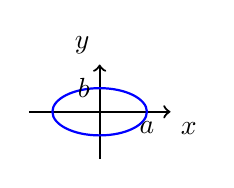
\begin{tikzpicture}[scale=0.3]
                \draw[thick,->] (-3,0) -- (3,0) node[anchor=north west] {$x$};
                \draw[thick,->] (0,-2) -- (0,2) node[anchor=south east] {$y$};
                \draw[thick,blue] (0,0) ellipse (2 and 1);
                \node[anchor=north] at (2,0) {$a$};
                \node[anchor=east] at (0,1) {$b$};
            \end{tikzpicture}

            \item Гипербола $\frac{x^2}{a^2} - \frac{y^2}{b^2} = 1$
            
            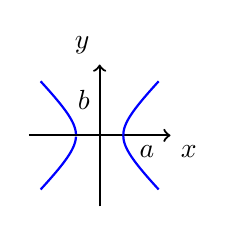
\begin{tikzpicture}[scale=0.3]
                \draw[thick,->] (-3,0) -- (3,0) node[anchor=north west] {$x$};
                \draw[thick,->] (0,-3) -- (0,3) node[anchor=south east] {$y$};
                \draw[thick,blue,domain=1.0:2.5,samples=100] plot (\x,{sqrt((\x)^2 - 1)});
                \draw[thick,blue,domain=1.0:2.5,samples=100] plot (\x,{-sqrt((\x)^2 - 1)});
                \draw[thick,blue,domain=-2.5:-1.0,samples=100] plot (\x,{sqrt((\x)^2 - 1)});
                \draw[thick,blue,domain=-2.5:-1.0,samples=100] plot (\x,{-sqrt((\x)^2 - 1)});
                \node[anchor=north] at (2,0) {$a$};
                \node[anchor=east] at (0,1.5) {$b$};
            \end{tikzpicture}

        \item $y - ax^2 = 0$
        
            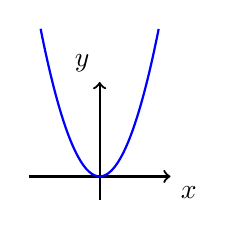
\begin{tikzpicture}[scale=0.3]
                \draw[thick,->] (-3,0) -- (3,0) node[anchor=north west] {$x$};
                \draw[thick,->] (0,-1) -- (0,4) node[anchor=south east] {$y$};
                \draw[thick,blue,domain=-2.5:2.5,samples=100] plot (\x,{(\x)^2});
            \end{tikzpicture}

        \item Пара пересекающихся прямых $\frac{x^2}{a^2} - \frac{y^2}{b^2} = 0$
        
        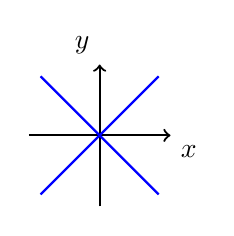
\begin{tikzpicture}[scale=0.3]
            \draw[thick,->] (-3,0) -- (3,0) node[anchor=north west] {$x$};
            \draw[thick,->] (0,-3) -- (0,3) node[anchor=south east] {$y$};
            \draw[thick,blue] (-2.5,-2.5) -- (2.5,2.5);
            \draw[thick,blue] (-2.5,2.5) -- (2.5,-2.5);
        \end{tikzpicture}

        \item Пара $\parallel$ прямых $(x - a)(x - b) = 0$
        
        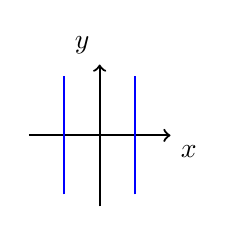
\begin{tikzpicture}[scale=0.3]
            \draw[thick,->] (-3,0) -- (3,0) node[anchor=north west] {$x$};
            \draw[thick,->] (0,-3) -- (0,3) node[anchor=south east] {$y$};
            \draw[thick,blue] (-1.5,-2.5) -- (-1.5,2.5);
            \draw[thick,blue] (1.5,-2.5) -- (1.5,2.5);
        \end{tikzpicture}

        \item Прямая $ax + by + c = 0$
        
        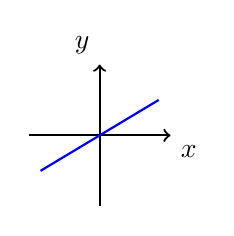
\begin{tikzpicture}[scale=0.3]
            \draw[thick,->] (-3,0) -- (3,0) node[anchor=north west] {$x$};
            \draw[thick,->] (0,-3) -- (0,3) node[anchor=south east] {$y$};
            \draw[thick,blue] (-2.5,-1.5) -- (2.5,1.5);
        \end{tikzpicture}

        \item Пустое множество $\frac{x^2}{a^2} + \frac{y^2}{b^2} = -1$ 
        \item Точка $\frac{x^2}{a^2} + \frac{y^2}{b^2} = 0$ 
        \item Все $\R^2$ $a = 0;\ L = 0;\ c = 0 \Rightarrow 0 = 0$
    \end{enumerate}
\end{Example}

\begin{defin}{}
    Поверхность $P$ называется центральное, если она имеет центр симметрии, то есть \\ $\exists x_0 \in \R^n : x_0 + y \in P \Leftrightarrow x_0 - y \in P$
\end{defin}

\begin{Example}{}
    $x_0 = 0 \Rightarrow Y \in P \Leftrightarrow -Y \in P$ 
\end{Example}

\begin{theo}{Утверждение}
    $L = 0 \Rightarrow P$ -- симметрично относительно 0, т.е. $Q(x) = Q(-x)$

    В содержательных случаях это равносильно

    $P$ -- поверхность. Существует ли такая замена координат, после которой $L = 0$?

    Сделаем перенос на $D$ (см. выше)

    $L \mapsto 2D^TQ + L$

    $L^T \mapsto 2QD + L^T$

    \begin{enumerate}
        \item Пусть $Q$ -- невырожденная квадартичная форма. Т.е. $\exists D : QD = \frac{-L^T}{2} \Rightarrow L_{new} = 0$
        
        Получаем уравнение $X^TQX = -C$

        Существует ортогональное преобразование $Q \mapsto \tilde{Q} = \begin{pmatrix}
            a_1 & \ldots & 0 \\
            \vdots & \ddots & \vdots \\
            0 & \ldots & a_n 
        \end{pmatrix}$

        $\Rightarrow$ уравнение превращается в $a_1x_1^2 + \ldots + a_nx_n^2 = const$

        Если $x' = \sqrt{|a_i|}x$, то получим $\pm x_1^2 \pm \ldots \pm x_n^2 = c$

        \begin{Example}{}
            $n = 2$

            $\pm x_1^2 \pm x_2^2 = 1$ -- эллипс/гипербола/$\varnothing$
        
            $\pm x_1^2 \pm x_2^2 = 0$ -- точка/две прямые
        \end{Example}

        \item $Q$ вырождена, $\frac{-L^T}{2} \in \im Q \Rightarrow$ можем сделать $L = 0$ и диагонализировать $Q$ ортогональным преобразованием $\Rightarrow a_1x_1^2 + \ldots + a_kx_k^2 = -c\ k < n$
        
        \begin{Example}{}
            $n = 2$

            $ax^2 = 0$ -- прямая

            $0 = 0$ -- $\R^2$
        \end{Example}

        \item $\frac{-L^T}{2} \notin \im Q \Rightarrow$ не можем сделать $L = 0$, <<остается только плакать и жаловаться на жизнь>>
        
        Диагонализуем $Q$

        $a_1x_1^2 \ldots + a_kx_k^2 + b_1x_1 + \ldots + b_nx_n + c = 0;\ k < n$

        Если $b_{k + 1} + \ldots + b_n = 0$, то получим $\sum\limits_{i = 1}^k (a_ix_i^2 + b_ix_i) + c = 0$, т.е. $\sum a_ix_i'^2 + c' = 0$

        Пусть НУО $b_{k + 1} \neq 0$, тогда $x_i' = x_i\ \forall i \neq k + 1$

        $x_{k + 1}' = \sum b_ix_i$

        Получим точно обратимую матрицу, т.е. невырожденная замена (можно сделать ортогональную)

        В новых координатах $a_1x_1'^2 + \ldots + a_kx_k'^2 + x_{k + 1}' + c = 0$

        $x_{k + 1}'' = x_{k + 1}' + c$

        Вывод: любая нецентральная квадратичная поверхность заменой координат приводится к уравнению $x_{k + 1} = \sum a_ix_i^2$
    \end{enumerate}
\end{theo}

\begin{Example}{}
    В случае $n = 2$

    $x_1 = ax_1^2$ -- парабола

    $x_1 = 0$ -- прямая 
\end{Example}

\begin{nota}{Обязательно посмотрите запись там много рисунков!}
    На самом деле эллипс, гипербола и парабола -- это одно и то же 

    Рассмотрим $\R^3 = \{ \begin{pmatrix}
        x \\
        y \\
        z 
    \end{pmatrix} \mid x, y, z \in \R \}$

    На $\R^3 \setminus \{0\}$ зададим $\sim$

    $\begin{pmatrix}
        x \\
        y \\
        z 
    \end{pmatrix} \sim \begin{pmatrix}
        x' \\
        y' \\
        z'
    \end{pmatrix}$, если $\exists k \neq 0 : \begin{cases}
        x' = kx \\
        y' = ky \\
        z' = kz
    \end{cases}$

    $(\R^3 \setminus \{0\})/_{\sim} = \R p^2$ -- проективная плоскость

    $\R^2 \sim \{ \begin{pmatrix}
        x \\
        y \\
        1
    \end{pmatrix} \mid x, y \in \R \} = L$

    Существует биекция $L \leftrightarrow \{ \ol{\begin{pmatrix}
        x \\
        y \\
        z 
    \end{pmatrix}} \mid z \neq 0 \}$

    Можно представить $\R p^2 = L \cup \{ \overline{\begin{pmatrix}
        x \\
        y \\
        0
    \end{pmatrix}}\}$ -- эти классы соответствуют направлениям в плоскости $L$

    $\ol{\begin{pmatrix}
        x \\
        y \\
        0
    \end{pmatrix}}$ -- бесконечно удаленная точка в направлении вектора $x, y$
\end{nota}

\end{document}